\chapter{Resultados Experimentais} \label{chap:resexp}


Os testes desta secção têm como objetivo encontrar o melhor detetor / descritor / matcher, determinando a robustez do subsistema de localização para o ruído, iluminação variante e rotação.

Os parâmetros utilizados nos vários detetores, para limitar o número de pontos característicos, são definidos com base no valor médio de intensidade da imagem. Desta forma, os detetores trabalham sob várias condições de brilho.

Para obter resultados constantes, a plataforma ROS permite ao usuário reproduzir uma sequência de mensagens nas mesmas condições em que foram adquiridas. Esta funcionalidade permite ao desenvolvedor resultados constantes, ou seja, diferentes combinações de parâmetros podem ser testadas para a mesma entrada .

\section{Calibração da câmara}

Como mencionado anteriormente, no capítulo ~\ref{section:Intrin}, as câmaras e lentes têm que ser calibradas para não causar erros de distorção nos resultados finais. 

\begin{figure}[h!]  %colocar figura a seguir ao texto anterior
	\centering
	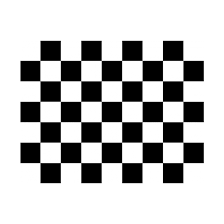
\includegraphics[width=0.4\linewidth]{checkboard.png} 
	\caption{Quadrado de xadrez para calibrar câmara.}
	\label{fig:checkboard}  %30 years. Figure 3 a)
\end{figure}

Desta forma, é usado o algoritmo desenvolvido em ~\cite{piCam}, que se baseia no uso de um quadrado de xadrez, figura ~\ref{fig:checkboard}. Este é composto por quadrados com a mesma largura, que devido à sua estrutura em  xadrez, facilita a determinação de pontos de interseção \ cruzamento. Com estes pontos é possível criar linhas com tamanhos conhecidos e através destas obter os parâmetros intrínsecos da câmara-lente. 



A figura ~\ref{fig:imgcheckboard} ilustra a calibração da devida câmara do raspberry pi com uma lente olho de peixe \textit{full-frame}. O resultado final é a matriz de parâmetros intrínsecos composta por : \[ \left[ \begin{array}{ccc}
603.104 & 0 & 651.767 \\ 
0 & 601.316 & 337.810 \\ 
0 & 0 & 1
\end{array} \right] \] e a matriz de parâmetros de distorção \[ \left[\begin{array}{ccccc}
-0.308 & 0.0729 & 0.00208 & -0.00157 & 0 
\end{array} \right] \]

\begin{figure}[h!]  %colocar figura a seguir ao texto anterior
	\centering
	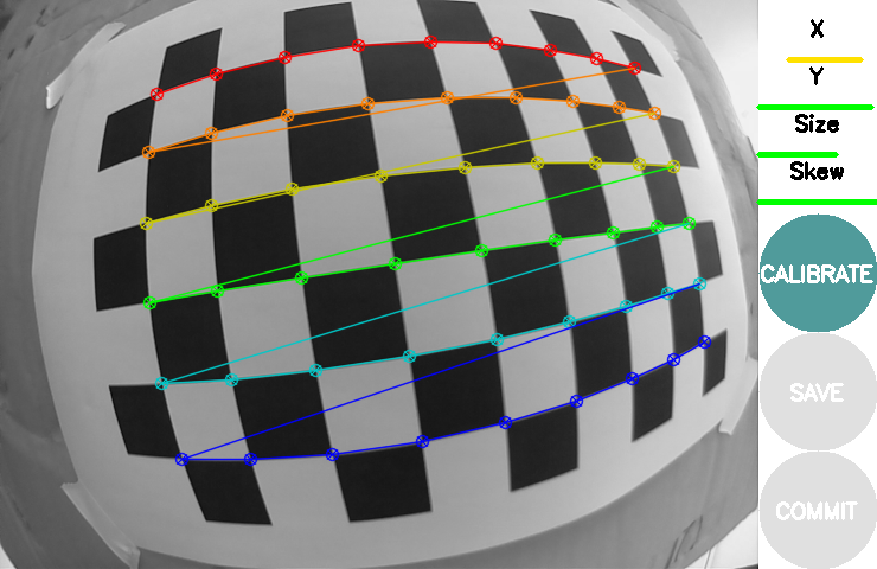
\includegraphics[width=0.6\linewidth]{imgcheckboard.png} 
	\caption{Imagem da calibração dos parâmetros da câmara.}
	\label{fig:imgcheckboard}  %30 years. Figure 3 a)
\end{figure}


Desta forma, é possível retirar a distorção de uma imagem lente olho de peixe . 



Como ilustrado na figura ~\ref{fig:FishEyeN} a imagem possui a distorção de lente olho de peixe  de uma grande ocular .  Removida a distorção da imagem é obtida a figura ~\ref{fig:FishEyeUndist}, na qual é reduzido o ângulo de abertura.

\begin{figure}[h!]
	\centering
	\subfloat[\label{fig:FishEyeN}]{
		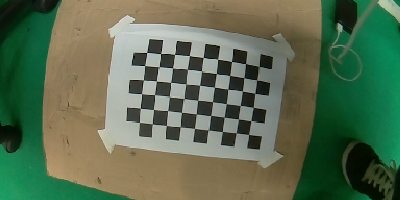
\includegraphics[width=0.46\textwidth]{ImagemFishEye.png}}
	\qquad
	\subfloat[\label{fig:FishEyeUndist}]{
		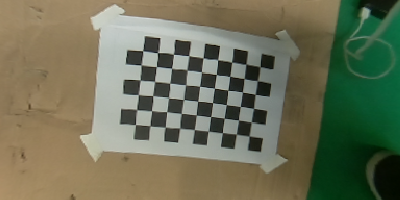
\includegraphics[width=0.46\textwidth]{ImagemFishEyeUndist.png}}
	\caption{Diferença entre ângulos de abertura em imagem com e sem distorção.}\label{fig:FisheEye}
\end{figure}


Quando removida a distorção da imagem o ângulo de abertura diminui, mas continua sendo maior que o ângulo de uma câmara sem lente olho de peixe, como ilustrado na figura ~\ref{fig:ImageNorm}. Esta foi capturada com a mesma câmara, sem lente olho de peixe, e à mesma distância do quadrado de xadrez.

\begin{figure}[h!]
	\centering
	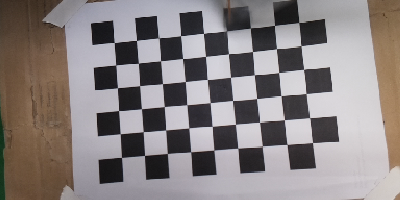
\includegraphics[width=0.5\textwidth]{ImagemNormal.png}
	\caption{Imagem sem lente olho de peixe.}
	\label{fig:ImageNorm}
\end{figure}







\section{Diferença entre detetores de características}

Na presente dissertação, serão comparados 4 detetores de características (FAST, SIFT, SURF, HARRIS), explícitos em  ~\ref{detCar}. Os testes são realizados num ambiente agrícola para maior coerência com a ambiente na qual a dissertação está envolvida, como ilustrado na figura ~\ref{fig:metodosALL}.


%\begin{figure}[h!]  %colocar figura a seguir ao texto anterior
%	\begin{center}
%	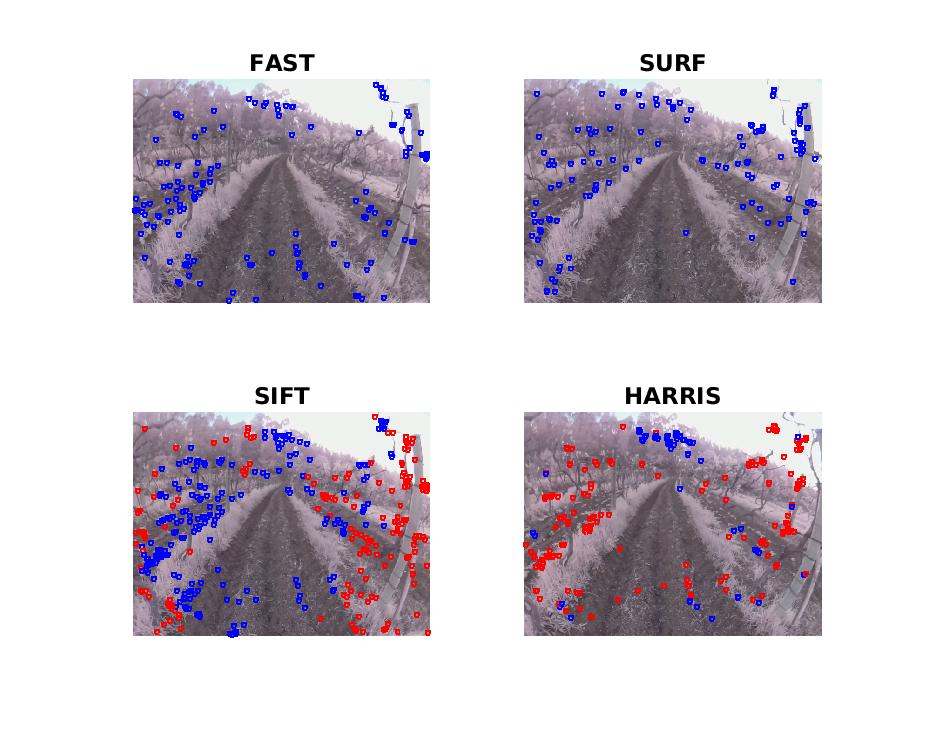
\includegraphics[width=0.8\linewidth]{FAST_SURF_SIFT_HARRIS.eps} 
%	\caption{Distribuição dos pontos caracterisiticos para os quatro detetores de características, FAST, SURF, SIFT, HARRIS.}
%	\label{fig:4metodos}  %30 years. Figure 3 a)
%	\end{center}
%\end{figure}


\begin{figure}[h!]
	\centering
	\subfloat[FAST\label{fig:metodosFAST}.]{
		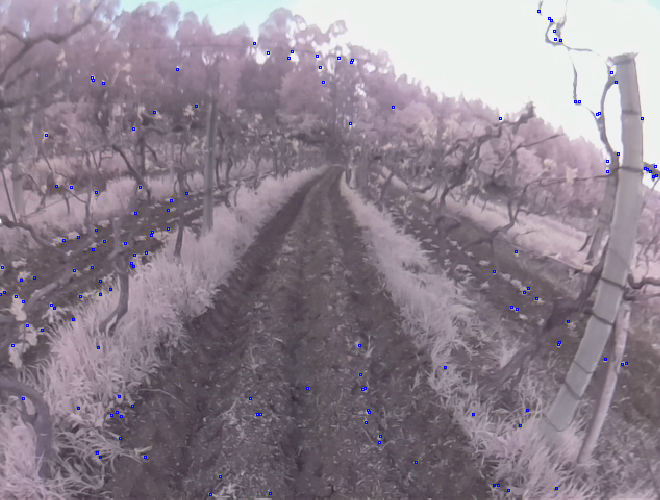
\includegraphics[width=0.45\textwidth]{metodosFAST.png}}
	\qquad
	\subfloat[SURF\label{fig:metodosSURF}.]{
		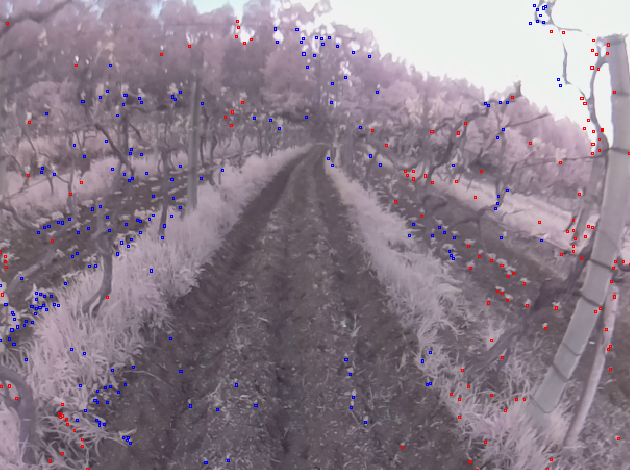
\includegraphics[width=0.46\textwidth]{metodosSURF.png}}

	\subfloat[SIFT\label{fig:metodosSIFT}.]{
		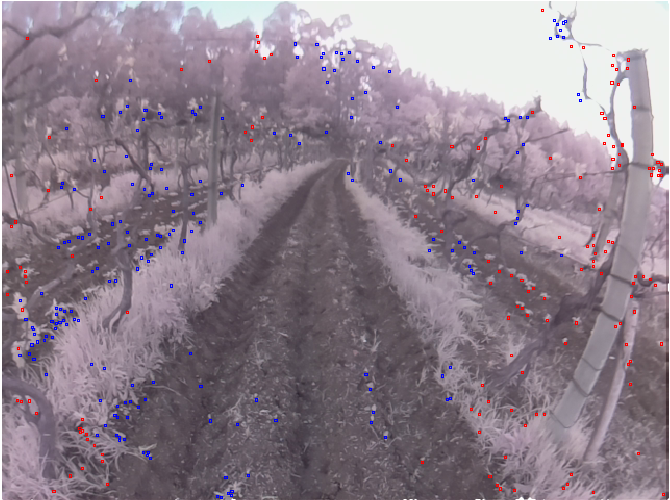
\includegraphics[width=0.45\textwidth]{metodosSIFT.png}}
	\qquad
	\subfloat[HARRIS\label{fig:metodosHARRIS}.]{
		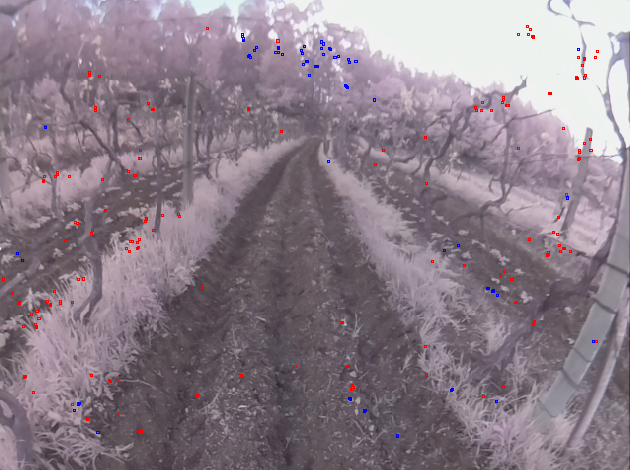
\includegraphics[width=0.45\textwidth]{metodosHARRIS.png}}
	\caption{Distribuição dos pontos característicos para os quatro detetores de características}\label{fig:metodosALL}
\end{figure}


De notar, que os pontos azuis são pontos de características que têm correspondências corretas no próximo frame e os pontos vermelhos são \textit{outliers}, pontos com correspondência de características erradas e/ou sem correspondências.

Os métodos têm as suas diferenças, desde logo a quantidade dos pontos com correspondência no frame seguinte. Desta forma, o método HARRIS e o método SIFT, são pouco eficazes. O primeiro pelo facto de apresentar poucas correspondências e o segundo devido a eliminar muitos pontos característicos de curta distância. A distribuição dos pontos característicos é favorável no método SURF, FAST e SIFT, sendo o primeiro o melhor. O método SURF apresenta maior seleção de pontos nas videiras, sendo estes mais estáveis e recomendados, devido ao ambiente vincula. Em termos de quantidade de pontos, o método SIFT apresenta um elevado número, o que implica maior tempo de processamento e maior número de frames perdidos entre ciclos. Esta quantidade podia ser diminuída, mas em cenários mais precários o algoritmo fica sujeito a encontrar um número reduzido de pontos característicos que impossibilitem o funcionamento do algoritmo. 

Assim, o método HARRIS é o menos eficaz, devido a fraca qualidade e distribuição dos pontos característicos. O método SIFT tem um grande tempo de processamento, que caso a velocidade do robô seja baixa é uma solução plausível, pelo facto ter uma elevada quantidade de pontos característicos e uma boa distribuição. Por fim, o método FAST e SURF são os mais indicativos. Sendo, o último com melhor distribuição  dos pontos característicos. 


\section{Comparação das combinações}\label{sec:Tempos}


Como explicito no capítulo ~\ref{chap:odometria visual}, existem vários detetores de características, descritores de características e métodos de associação de características. Nesta dissertação são usados 4 detetores de características ( FAST, HARRIS, SIFT e SURF ), 3 descritores de característica ( ORB, SIFT e SURF)  e 2 métodos de associação de características ( FLANN e Brute-Force)  totalizando 24 combinações.

Os métodos são comparados pelos seguintes critérios :
\begin{itemize}
	\item \textbf{Imagens} - número de imagens ( \textit{frames}) processadas.
	\item \textbf{Tempo} - mínimo, máximo e média de tempo nos ciclos de processamento, em segundos.
	\item \textbf{Imagens perdidas (\textit{Lost Frames})} - quantidade de imagens perdidas(não analisadas) entre ciclos de processamento.
	\item \textbf{Número} \textbf{de} \textbf{pontos} \textbf{característicos} - quantidade mínima, máxima e média de pontos característicos nos ciclos de processamento.
\end{itemize}


De forma a obter resultados coerentes é utilizado sempre a mesma movimentação, ficheiro \textit{bag}, em todos os teste. 


%\begin{figure}[h!] %colocar figura a seguir ao texto anterior
%	\begin{center}
%		\leavevmode		
%		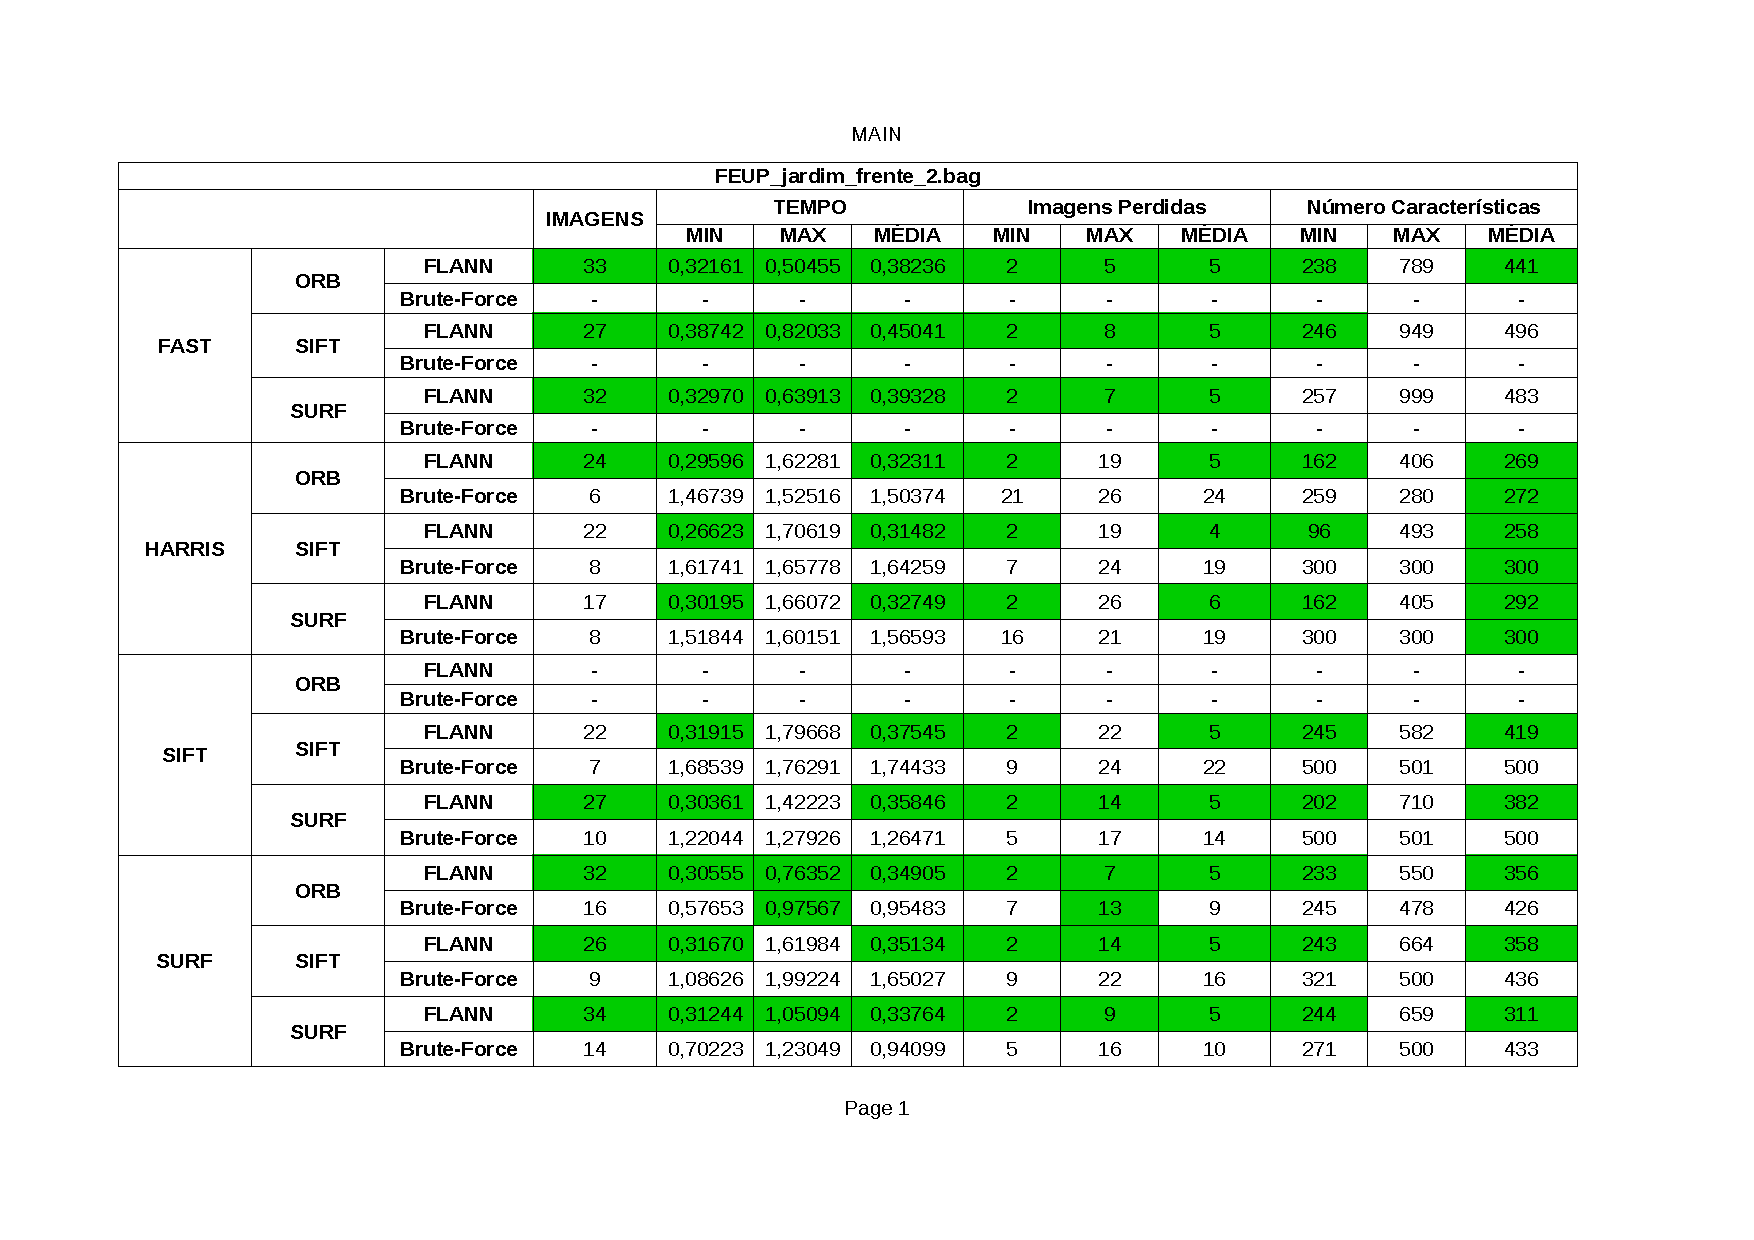
\includegraphics[width=1\textwidth]{compararMetodos.pdf}
%		\caption{Tabela de comparação das combinações dos métodos.}
%		\label{fig:compMet}
%	\end{center}
%\end{figure}


% Please add the following required packages to your document preamble:
% \usepackage{multirow}
% \usepackage[table,xcdraw]{xcolor}
% If you use beamer only pass "xcolor=table" option, i.e. \documentclass[xcolor=table]{beamer}
\begin{table}[h!]
	\centering
	\caption{Tabela de comparação das combinações dos métodos.}
	\label{tab:compMet}
	\resizebox{\textwidth}{!}{\begin{tabular}{|c|c|c|c|c|c|c|c|c|c|c|c|c|}
				\hline
				\multicolumn{13}{|c|}{FEUP\_jardim\_frente\_2.bag}                                                                                                                                                                                                                                                                                                        \\ \hline
				\multicolumn{3}{|c|}{}                                          &                            & \multicolumn{3}{c|}{TEMPO (s)}                                                                          & \multicolumn{3}{c|}{IMAGENS PERDIDAS}                                              & \multicolumn{3}{c|}{NÚMERO CARACTERÍSTICAS}                     \\ \cline{5-13} 
				\multicolumn{3}{|c|}{\multirow{-2}{*}{}}                        & \multirow{-2}{*}{IMAGENS}  & MIN                             & MAX                             & MÉDIA                           & MIN                       & MAX                        & MÉDIA                     & MIN                         & MAX & MÉDIA                       \\ \hline
				&                        & FLANN       & \cellcolor[HTML]{32CB00}33 & \cellcolor[HTML]{32CB00}0,32161 & \cellcolor[HTML]{32CB00}0,50455 & \cellcolor[HTML]{32CB00}0,38236 & \cellcolor[HTML]{32CB00}2 & \cellcolor[HTML]{32CB00}5  & \cellcolor[HTML]{32CB00}5 & \cellcolor[HTML]{32CB00}238 & 789 & \cellcolor[HTML]{32CB00}441 \\ \cline{3-13} 
				& \multirow{-2}{*}{ORB}  & Brute-Force & -                          & -                               & -                               & -                               & -                         & -                          & -                         & -                           & -   & -                           \\ \cline{2-13} 
				&                        & FLANN       & \cellcolor[HTML]{32CB00}27 & \cellcolor[HTML]{32CB00}0,38742 & \cellcolor[HTML]{32CB00}0,82033 & \cellcolor[HTML]{32CB00}0,45041 & \cellcolor[HTML]{32CB00}2 & \cellcolor[HTML]{32CB00}8  & \cellcolor[HTML]{32CB00}5 & \cellcolor[HTML]{32CB00}246 & 949 & 496                         \\ \cline{3-13} 
				& \multirow{-2}{*}{SIFT} & Brute-Force & -                          & -                               & -                               & -                               & -                         & -                          & -                         & -                           & -   & -                           \\ \cline{2-13} 
				&                        & FLANN       & \cellcolor[HTML]{32CB00}32 & \cellcolor[HTML]{32CB00}0,32970 & \cellcolor[HTML]{32CB00}0,63913 & \cellcolor[HTML]{32CB00}0,39328 & \cellcolor[HTML]{32CB00}2 & \cellcolor[HTML]{32CB00}7  & \cellcolor[HTML]{32CB00}5 & 257                         & 999 & 483                         \\ \cline{3-13} 
				\multirow{-6}{*}{FAST}   & \multirow{-2}{*}{SURF} & Brute-Force & -                          & -                               & -                               & -                               & -                         & -                          & -                         & -                           & -   & -                           \\ \hline
				&                        & FLANN       & \cellcolor[HTML]{32CB00}24 & \cellcolor[HTML]{32CB00}0,29596 & 1,62281                         & \cellcolor[HTML]{32CB00}0,32311 & \cellcolor[HTML]{32CB00}2 & 19                         & \cellcolor[HTML]{32CB00}5 & \cellcolor[HTML]{32CB00}162 & 406 & \cellcolor[HTML]{32CB00}269 \\ \cline{3-13} 
				& \multirow{-2}{*}{ORB}  & Brute-Force & 6                          & 1,46739                         & 1,52516                         & 1,50374                         & 21                        & 26                         & 24                        & 259                         & 280 & \cellcolor[HTML]{32CB00}272 \\ \cline{2-13} 
				&                        & FLANN       & 22                         & \cellcolor[HTML]{32CB00}0,26623 & 1,70619                         & \cellcolor[HTML]{32CB00}0,31482 & \cellcolor[HTML]{32CB00}2 & 19                         & \cellcolor[HTML]{32CB00}4 & \cellcolor[HTML]{32CB00}96  & 493 & \cellcolor[HTML]{32CB00}258 \\ \cline{3-13} 
				& \multirow{-2}{*}{SIFT} & Brute-Force & 8                          & 1,61741                         & 1,65778                         & 1,64259                         & 7                         & 24                         & 19                        & 300                         & 300 & \cellcolor[HTML]{32CB00}300 \\ \cline{2-13} 
				&                        & FLANN       & 17                         & \cellcolor[HTML]{32CB00}0,30195 & 1,66072                         & \cellcolor[HTML]{32CB00}0,32749 & \cellcolor[HTML]{32CB00}2 & 26                         & \cellcolor[HTML]{32CB00}6 & \cellcolor[HTML]{32CB00}162 & 405 & \cellcolor[HTML]{32CB00}292 \\ \cline{3-13} 
				\multirow{-6}{*}{HARRIS} & \multirow{-2}{*}{SURF} & Brute-Force & 8                          & 1,51844                         & 1,60151                         & 1,56593                         & 16                        & 21                         & 19                        & 300                         & 300 & \cellcolor[HTML]{32CB00}300 \\ \hline
				&                        & FLANN       & -                          & -                               & -                               & -                               & -                         & -                          & -                         & -                           & -   & -                           \\ \cline{3-13} 
				& \multirow{-2}{*}{ORB}  & Brute-Force & -                          & -                               & -                               & -                               & -                         & -                          & -                         & -                           & -   & -                           \\ \cline{2-13} 
				&                        & FLANN       & 22                         & \cellcolor[HTML]{32CB00}0,31915 & 1,79668                         & \cellcolor[HTML]{32CB00}0,37545 & \cellcolor[HTML]{32CB00}2 & 22                         & \cellcolor[HTML]{32CB00}5 & \cellcolor[HTML]{32CB00}245 & 582 & \cellcolor[HTML]{32CB00}419 \\ \cline{3-13} 
				& \multirow{-2}{*}{SIFT} & Brute-Force & 7                          & 1,68539                         & 1,76291                         & 1,74433                         & 9                         & 24                         & 22                        & 500                         & 501 & 500                         \\ \cline{2-13} 
				&                        & FLANN       & \cellcolor[HTML]{32CB00}27 & \cellcolor[HTML]{32CB00}0,30361 & 1,42223                         & \cellcolor[HTML]{32CB00}0,35846 & \cellcolor[HTML]{32CB00}2 & \cellcolor[HTML]{32CB00}14 & \cellcolor[HTML]{32CB00}5 & \cellcolor[HTML]{32CB00}202 & 710 & \cellcolor[HTML]{32CB00}382 \\ \cline{3-13} 
				\multirow{-6}{*}{SIFT}   & \multirow{-2}{*}{SURF} & Brute-Force & 10                         & 1,22044                         & 1,27926                         & 1,26471                         & 5                         & 17                         & 14                        & 500                         & 501 & 500                         \\ \hline
				&                        & FLANN       & \cellcolor[HTML]{32CB00}32 & \cellcolor[HTML]{32CB00}0,30555 & \cellcolor[HTML]{32CB00}0,76352 & \cellcolor[HTML]{32CB00}0,34905 & \cellcolor[HTML]{32CB00}2 & \cellcolor[HTML]{32CB00}7  & \cellcolor[HTML]{32CB00}5 & \cellcolor[HTML]{32CB00}233 & 550 & \cellcolor[HTML]{32CB00}356 \\ \cline{3-13} 
				& \multirow{-2}{*}{ORB}  & Brute-Force & 16                         & 0,57653                         & \cellcolor[HTML]{32CB00}0,97567 & 0,95483                         & 7                         & \cellcolor[HTML]{32CB00}13 & 9                         & 245                         & 478 & 426                         \\ \cline{2-13} 
				&                        & FLANN       & \cellcolor[HTML]{32CB00}26 & \cellcolor[HTML]{32CB00}0,31670 & 1,61984                         & \cellcolor[HTML]{32CB00}0,35134 & \cellcolor[HTML]{32CB00}2 & \cellcolor[HTML]{32CB00}14 & \cellcolor[HTML]{32CB00}5 & \cellcolor[HTML]{32CB00}243 & 664 & \cellcolor[HTML]{32CB00}358 \\ \cline{3-13} 
				& \multirow{-2}{*}{SIFT} & Brute-Force & 9                          & 1,08626                         & 1,99224                         & 1,65027                         & 9                         & 22                         & 16                        & 321                         & 500 & 436                         \\ \cline{2-13} 
				&                        & FLANN       & \cellcolor[HTML]{32CB00}34 & \cellcolor[HTML]{32CB00}0,31244 & \cellcolor[HTML]{32CB00}1,05094 & \cellcolor[HTML]{32CB00}0,33764 & \cellcolor[HTML]{32CB00}2 & \cellcolor[HTML]{32CB00}9  & \cellcolor[HTML]{32CB00}5 & \cellcolor[HTML]{32CB00}244 & 659 & \cellcolor[HTML]{32CB00}311 \\ \cline{3-13} 
				\multirow{-6}{*}{SURF}   & \multirow{-2}{*}{SURF} & Brute-Force & 14                         & 0,70223                         & 1,23049                         & 0,94099                         & 5                         & 16                         & 10                        & 271                         & 500 & 433                         \\ \hline
		\end{tabular}}
\end{table}



A tabela ~\ref{tab:compMet} ilustra os resultados obtidos nos testes da bag \textit{$FEUP_jardim_frente_2.bag$}, num computador com as seguintes especificações :
\begin{itemize}
	\item CPU : AMD A4-5150M, 2700 MHz
	\item GPU : Radeon(tm) HD Graphics
	\item RAM : 3GB 
\end{itemize}


 As combinações representadas pelo símbolo \textbf{-} expressam testes na qual resultaram em erros, devido a um número baixo de características utilizadas ou poucas associações, durante um grande período de ciclos de processamento. De forma a melhor interpretação da tabela os valores com bons resultados estão coloridos de verde. 


Na coluna \textbf{Imagens} um valor elevado significa que o algoritmo é melhor. Nas colunas \textbf{mínimos, máximo e médios do Tempo, Imagens Perdidas e número de pontos característicos} quanto menor o valor melhor os resultados. 

Analisando a tabela, as combinações com o simbolo \textbf{-} ou sem células coloridas a verde são soluções ineficazes. A associação \textbf{Brute-Force} não tem nenhuma solução, devido ao tempo de processamento ser maior em relação ao método \textbf{FLANN} e, ainda, por apresentar menor coerência de correspondência de pontos característicos. Relativamente, aos detetores de \textbf{HARRIS} e \textbf{SIFT}são visíveis algumas soluções possíveis de utilizar. Contudo, apresentam parâmetros fracos, como a quantidade de imagens, tempo máximo e máxima quantidade de imagens perdidas. Quanto aos restantes métodos, todas as combinações são razoáveis para se implementar, mas importa salientar as combinações \textbf{FAST/ORB/FLANN} e \textbf{SURF/ORB/FLANN} pois tem os melhores parâmetros. Assim, estas últimas serão as utilizadas nos restantes testes.








\section{Testes}

De forma a validar o algoritmo de localização, os testes requerem a quantificação do erro. O erro é descrito como a diferença entre o valor real e o valor medido.

As coordenadas reais têm de ser obtidas através de um sensor externo, tal como, a laser baseado em localização, Odometria do robô ou mesmo uma fita métrica.Assim, os testes serão realizados no robô AgrobV16 e as coordenadas reais serão obtidas através da odometria das rodas, tópico \textit{$husky\_velocity\_controller/odom$}.

\subsection{Cinemática Agrob v16}

A cinemática é a área da Física que estuda o movimento dos corpos. Em robótica móvel, a cinemática estabelece relações entre o deslocamento (locomoção) do robô e a atuação a ele imposta. O robô AgrobV16 é utilizado nos teste, realizados, de forma a conseguir obter uma trajetória com maior precisão e ter uma variável de comparação, a odometria das rodas do robô, designada  Odometria das rodas, nomeada Odometria Husky. 

A cinemática direta estabelece modelos que estimam o deslocamento do robô dada uma atuação, por exemplo, velocidades impostas às suas rodas. A cinemática reversa estabelece modelos que estimam a atuação necessária para que o robô realize o determinado deslocamento, por exemplo, percorrer uma trajetória. Os modelos cinemáticos são baseados em equações diferenciais de primeira ordem não lineares. Tais modelos, são linearizados no tempo quando utilizados em aplicações robótica.


O modelo não tem em conta a inércia do robô, deformações em sua estrutura, forças oriundas do deslocamento (atrito, escorregamento, etc.) e demais fatores internos e externos que possam afetar a locomoção.


O robô AgrobV16, figura ~\ref{fig:agrobv16}, possui 4 rodas com tração, mas a cinemática no centro de massa é equivalente à cinemática de tração diferencial. Um robô diferencial possui 2 rodas com tração independente e 1 ou mais pontos de contacto, usualmente proporcionados por rodas sem tração. Por outo lado o AgrobV16 possui 4 rodas de tração mas a tração é aos pares, resultando na equivalência de 2 rodas .


\begin{figure}[h!] %colocar figura a seguir ao texto anterior
	\begin{center}
		\leavevmode		
		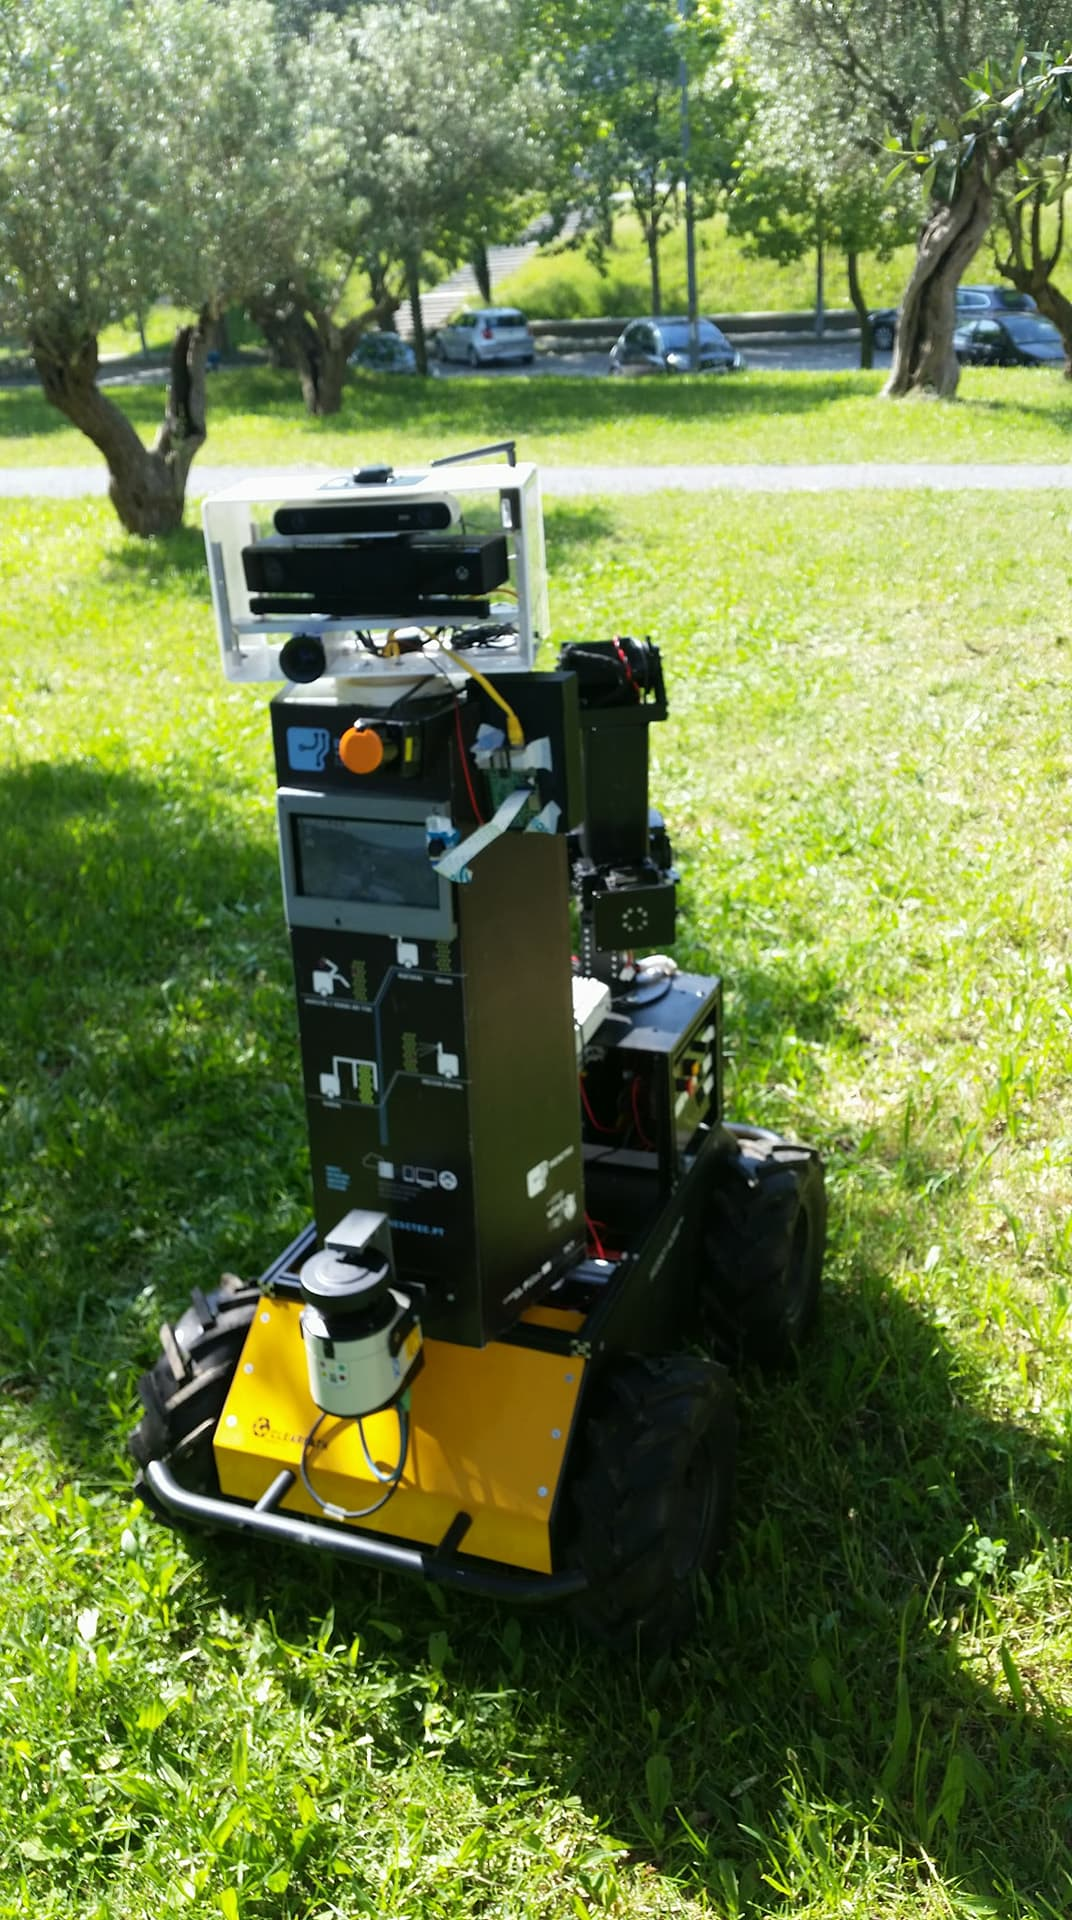
\includegraphics[width=0.5\textwidth]{testes/Agrobv16.jpg}
		\caption{Robô AgrobV16.}
		\label{fig:agrobv16}
	\end{center}
\end{figure}




Desta forma, a única forma de atuação em um robô diferencial, é pela imposição de velocidades independentes em cada roda. O robô diferencial possui estabilidade estática mas não é um robô omnidirecional, dado que é incapaz de se deslocar sobre o seu eixo transversal. Como ilustrado na figura ~\ref{fig:kinematicAgrob}, o centro de rotação do robô está localizado na intersecção dos eixos transversal (\textbf{$Y_R$}) e longitudinal (\textbf{$X_R$}).

\begin{figure}[h!] %colocar figura a seguir ao texto anterior
	\begin{center}
		\leavevmode		
		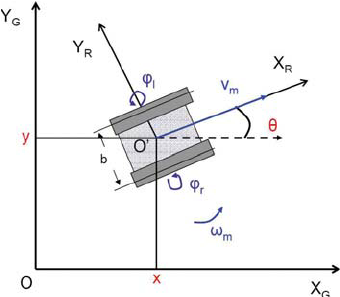
\includegraphics[width=0.5\textwidth]{kinematicAgrob.png}
		\caption{Modelo de Cinemática diferencial.}
		\label{fig:kinematicAgrob}
	\end{center}
\end{figure}


Considerando : 
\begin{itemize}
	\item \textbf{b} a distância entre rodas.
	\item \textbf{$\phi_r$} o raio da roda da direita.
	\item \textbf{$\phi_l$} o raio da roda da esquerda.
	\item \textbf{$v_r$} a velocidade da roda da direita.
	\item \textbf{$v_l$} a velocidade da roda da esquerda.
	\item \textbf{$v_m$} a velocidade linear do robô.
	\item \textbf{$\omega_m$} a velocidade angular do robô.
	\item $\textbf{$\theta$}$ o ângulo do robô, ângulo entre $v_m$ e eixo x.
\end{itemize}

Obtemos:
\[ \left\{\begin{array}{ccc}
v_1(t) = v_m(t) cos( \theta(t))\\ 
v_2(t) = v_m(t) sin( \theta(t))\\ 
\omega(t) = \omega(t)
\end{array}\right. \]

Originando: 

\[ v(t) = \frac{v_1(t)+v_2(t)}{2} \]

\[  \omega(t) = \frac{v_1(t)-v_2(t)}{b} \]

Em tempo discreto :

\[ d(i) = \frac{d_1(t)+d_2(t)}{2} \]

\[ \Delta \theta (i) = \frac{d_1(t)-d_2(t)}{b} \]

Sendo a posição seguinte dependente da posição atual, mais o deslocamento do robô em relação à velocidade resulta:

\[ \left\{\begin{array}{ccc}
x(i+1) = x(i) + d(i) cos( \theta(i) + \frac{\Delta \theta(i)}{2})\\ 
y(i+1) = y(i) + d(i) sin( \theta(i) + \frac{\Delta \theta(i)}{2})\\ 
\theta (i+1) = \theta (i) + \Delta \theta (i)
\end{array}\right. \]



\subsection{Setup Agrobv16}


Para a realização destes testes é necessário adaptar o robô Agrobv16, sendo adaptada uma câmara com lente olho de peixe e uma raspberry pi ao robô, como ilustra a figura ~\ref{fig:adptPicam}. No retângulo vermelho encontra-se a raspberry pi conectada com fios de alimentação, cabo ethernet, para comunicar com o ROS do robô (computador principal), e uma conexão à câmara, representada no retângulo verde.


\begin{figure}[h!] 
	\begin{center}
		\leavevmode		
		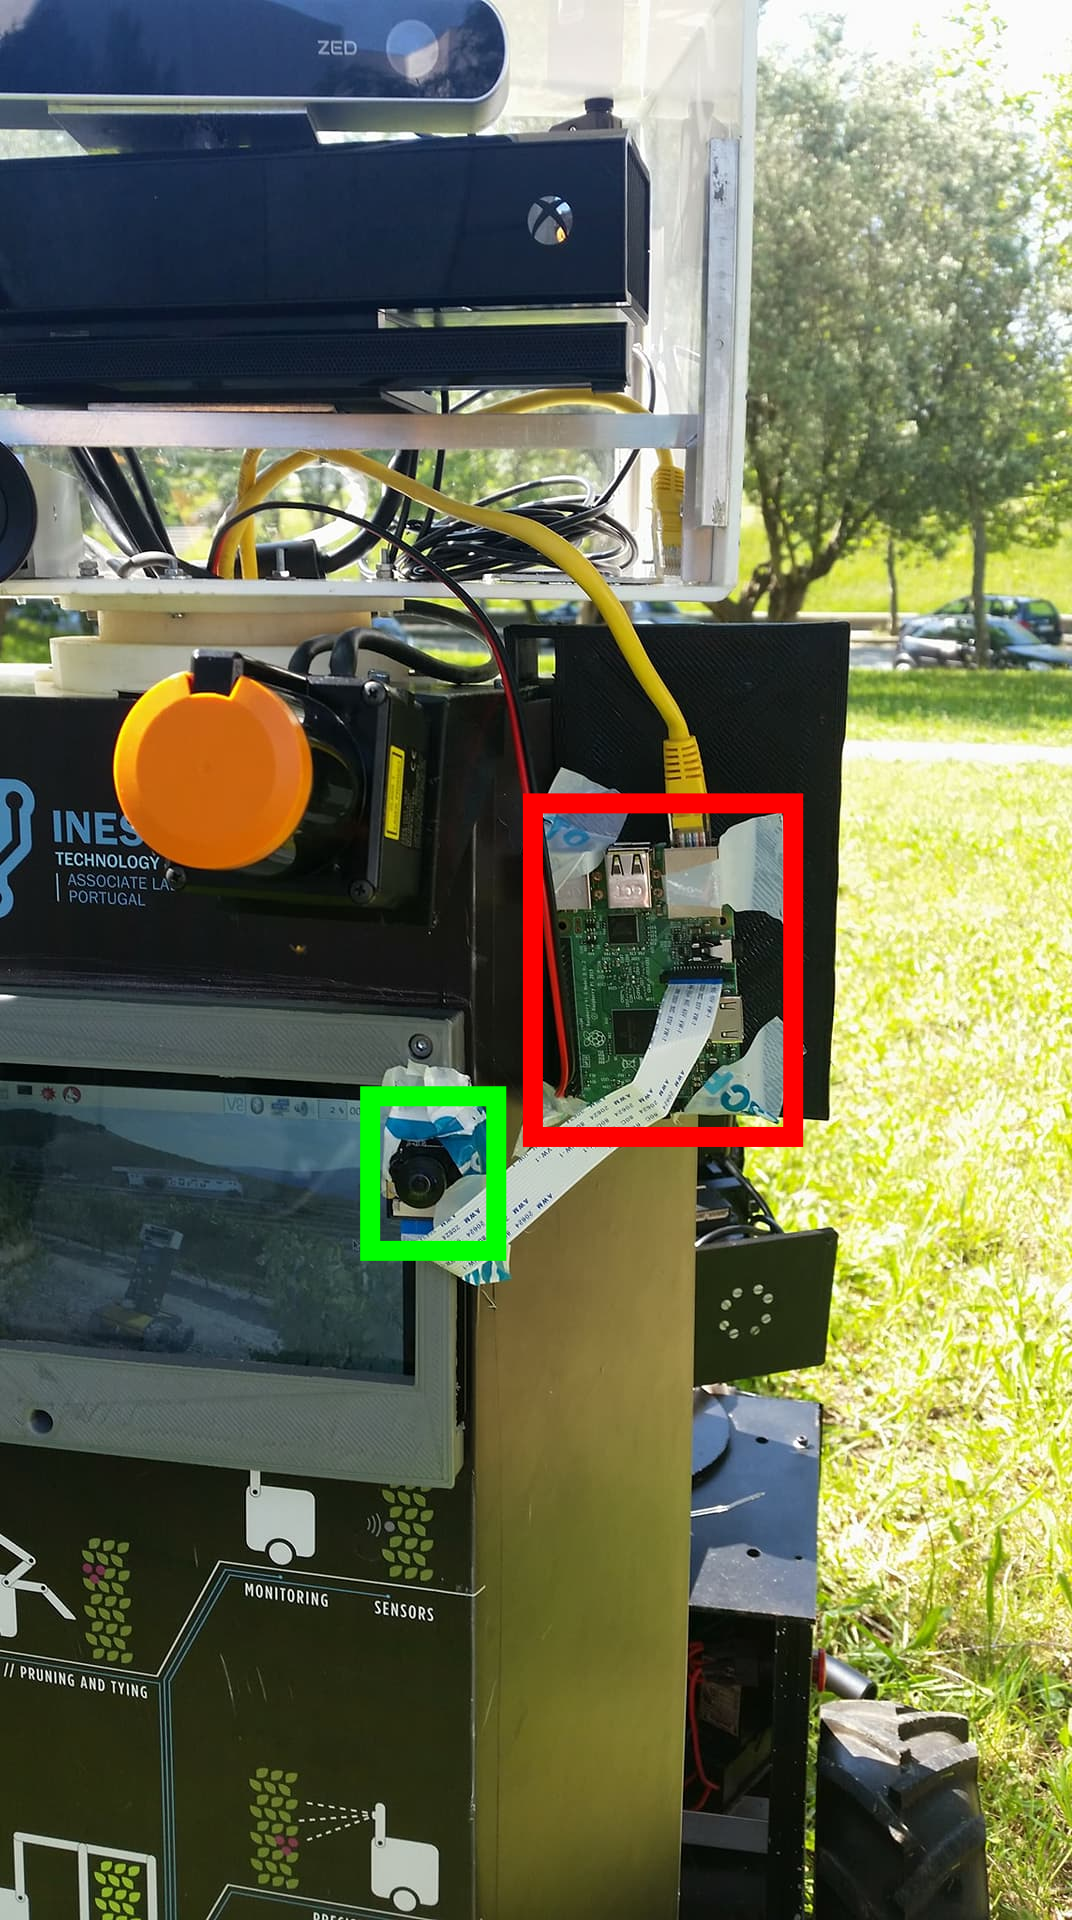
\includegraphics[width=0.35\textwidth]{testes/raspi_Agrob_edited.png}
		\caption{Setup no Agrobv16.}
		\label{fig:adptPicam}
	\end{center}
\end{figure}


\FloatBarrier
\subsection{Percursos e ambiente de teste}


Nesta subsecção são apresentados os percursos efetuados: estático, movimento em linha reta, movimento em L (semi-quadrado), percurso quadrangular e movimentos angulares de 90 graus. De salientar, que os percursos foram realizados com velocidades baixas. Assim, a câmara consegue extrair um maior número de características e consequentemente o erro da trajetória estimada será menor. 


O ambiente utilizado na realização dos testes foi no  jardim da FEUP, como ilustra a figura ~\ref{fig:ambTeste}. O ambiente mais conveniente seria numa vinha mas este não foi o possível, tendo-se optado pelo jardim da FEUP, ambiente mais propício para a realização dos testes. 


\begin{figure}[h!] 
	\begin{center}
		\leavevmode		
		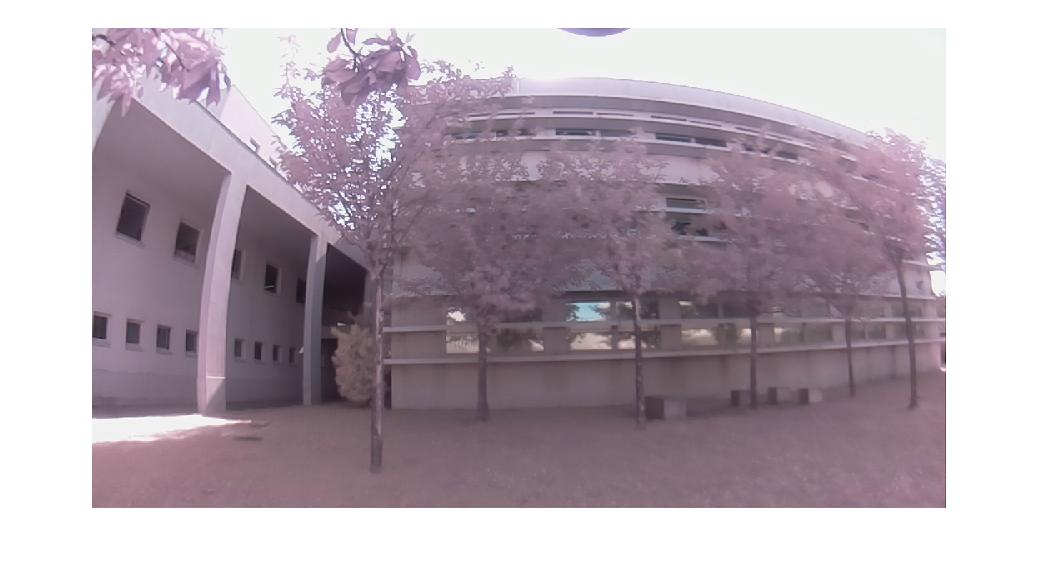
\includegraphics[width=0.8\textwidth]{ambTeste.jpg}
		\caption{Ambiente de testes na FEUP.}
		\label{fig:ambTeste}
	\end{center}
\end{figure}


Os teste foram todos realizados com o detetor de características SURF, descritor ORB e utilizado o método FLANN para correspondência de características. A escolha deste métodos é justificada na secção ~\ref{sec:Tempos}.


\subsection{Estático}\label{subsubsection:Estatico}

Com este teste é possível comprovar que o robô se encontra sempre na mesma posição, não existindo alterações no movimento, coordenadas x y e z, nem nas rotações, ângulos $\alpha$, $\beta$ e $\gamma$.



A partir da figura ~\ref{fig:trajRoboEst}  é possível analisar o posicionamento do robô, em que as coordenadas se  mantêm constantes, por ser um teste estático. Numa análise mais detalhada, verifica-se a existência de uma ligeira variação das coordenadas, que é considerada nula, figura ~\ref{fig:posEst}.


\begin{figure}[!htbp]
	\begin{center}
		\leavevmode		
		\includegraphics[width=0.65\textwidth]{testes/estatico/Trajetoria.eps}
		\caption{Trajetória do robô no teste estático.}
		\label{fig:trajRoboEst}
	\end{center}
\end{figure}



\begin{figure}[!htbp]
	\centering
	\subfloat[\label{fig:posVisoEst}]{
		\includegraphics[width=0.45\textwidth]{testes/estatico/PosicaoViso.eps}}
	\qquad
	\subfloat[\label{fig:posOdoEst}]{
		\includegraphics[width=0.45\textwidth]{testes/estatico/PosicaoOdo.eps}}
	\caption{Coordenadas x, y e z do robô no teste estático. a) Odometria Visual e b) Odometria das rodas do robô.}
	\label{fig:posEst}
\end{figure}

Em relação aos ângulos, estes também mantêm sempre o mesmo valor, figura ~\ref{fig:angEst}. De salientar, que na odometria das rodas, pelo tópico Husky o robô têm ângulos iniciais de  $\beta$ igual a 0 graus, $\gamma$ igual a -180 graus e $\alpha$ igual a 0 graus. Em relação aos ângulos da Odometria Visual é de notar que o valor de  $\alpha$ inicial é -23 graus, uma vez que não foi definida a posição inicial no início do teste, mas que não tem influência no resultado deste teste.

\begin{figure}[!htbp]
	\centering
	\subfloat[\label{fig:angVisoEst}]{
		\includegraphics[width=0.45\textwidth]{testes/estatico/AnglesViso.eps}}
	\qquad
	\subfloat[\label{fig:angOdoEst}]{
		\includegraphics[width=0.45\textwidth]{testes/estatico/AnglesOdo.eps}}
	\caption{Angulos $\alpha$, $\beta$ e $\gamma$ do robô no teste estático. a) Odometria Visual e b) Odometria das rodas do robô.}
	\label{fig:angEst}
\end{figure}


\FloatBarrier
\subsection{Movimento em linha reta reta}\label{subsubsection:Linha}

Com um movimento em linha reta é de esperar que a trajetória, apenas, varie uma coordenada da sua posição e mantenha sempre as mesmas coordenadas angulares.

\FloatBarrier
\subsubsection{Frente}\label{subsubsection:EmFrente}

Neste teste o robô desloca-se cerca de 3 metros em frente, movimento na coordenada x. 
Através da  figura ~\ref{fig:trajRobo3mFrente}, é possível analisar a trajetória obtida, em que  a Odometria das rodas do robô indica que o robô se deslocou cerca de 3 metros na coordenada x e a Odometria Visual mostra que o movimento foi até 32 numa escala indefinida. 

\begin{figure}[h!]
	\begin{center}
		\leavevmode		
		\includegraphics[width=0.65\textwidth]{testes/3mFrente/Trajetoria.eps}
		\caption{Trajetória do robô no movimento frente.}
		\label{fig:trajRobo3mFrente}
	\end{center}
\end{figure}

Analisando um movimento com maior precisão, ilustrado na figura ~\ref{fig:pos3mFrente} é possível comparar o trajeto na evolução das coordenadas. Assim, verifica-se que a figura  ~\ref{fig:posViso3mFrente} é visualmente idêntica à figura ~\ref{fig:posViso3mFrente}, em que aumenta sempre de forma semelhante. De salientar, apenas, uma variação pouco acentuada na coordenada x.


\begin{figure}[h!]
	\centering
	\subfloat[\label{fig:posViso3mFrente}]{
		\includegraphics[width=0.45\textwidth]{testes/3mFrente/PosicaoViso.eps}}
	\qquad
	\subfloat[\label{fig:posOdoEst2}]{
		\includegraphics[width=0.45\textwidth]{testes/3mFrente/PosicaoOdo.eps}}
	\caption{Coordenadas x, y e z do robô no movimento frente. a) Odometria Visual e b) Odometria das rodas do robô.}
	\label{fig:pos3mFrente}
\end{figure}


Quanto aos ângulos, estes mantêm-se nulos com esperado,  figura ~\ref{fig:ang3mFrente}. De notar que na figura ~\ref{fig:angOdo3mFrente} a variação do ângulo $\gamma$ se deve ao seu valor ser de 180 graus e o valor dos ângulos variar entre -180 graus e 180 graus, variando assim para -180 gruas.

\begin{figure}[h!]
	\centering
	\subfloat[\label{fig:angViso3mFrente}]{
		\includegraphics[width=0.45\textwidth]{testes/3mFrente/AnglesViso.eps}}
	\qquad
	\subfloat[\label{fig:angOdo3mFrente}]{
		\includegraphics[width=0.45\textwidth]{testes/3mFrente/AnglesOdo.eps}}
	\caption{Ângulos $\alpha$, $\beta$ e $\gamma$ do robô no movimento frente. a) Odometria Visual e b) Odometria das rodas do robô.}
	\label{fig:ang3mFrente}
\end{figure}

Para melhor interpretar os resultados obtidos foram realizados dois testes, para perceber a diferença nas escalas e a indefinição da escala da Odometria Visual. Esses mesmo testes serão realizados com igual distância percorridas, 10 centímetros, mas velocidades diferentes.


\subsubsection{Movimento 10 centímetros}\label{subcaption:10cm}

Para a realização deste teste é necessário um setup diferente do anterior. Assim, a câmara com lente olho de peixe é incorporada numa tábua de madeira, para realizar o movimento mais suave e sempre à mesma altura. Esta câmara é conectada a uma raspberry pi e, para que se possa  analisar as imagens capturadas. Na frente da câmara encontra-se uma folha branca com um quadrado preto para os detetores de características serem implementados. A figura ~\ref{fig:setup10cm} representa o setup implementado.

\begin{figure}[h!]
	\begin{center}
		\leavevmode		
		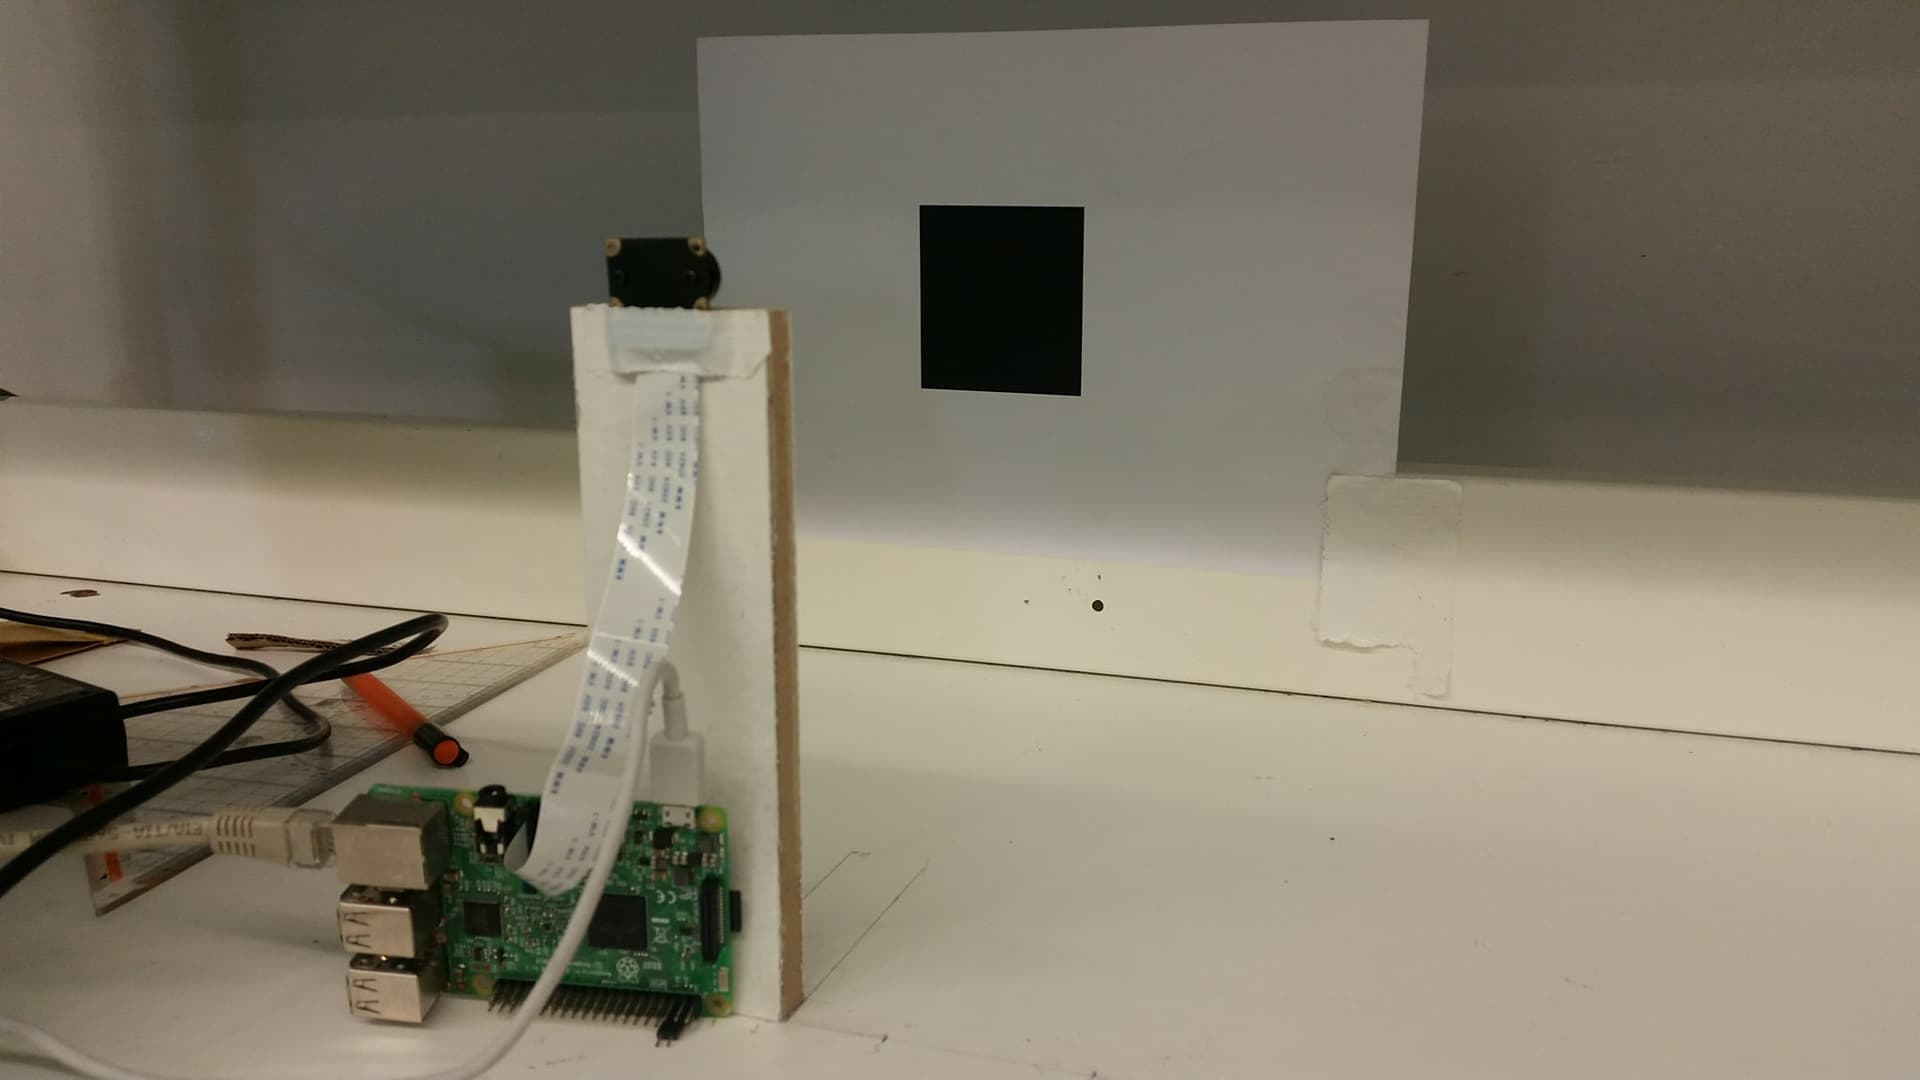
\includegraphics[width=0.65\textwidth]{testes/raspi_10cm.jpg}
		\caption{Setup no movimento de 10 centímetros.}
		\label{fig:setup10cm}
	\end{center}
\end{figure}
 


Primeiramente, análise as diferenças  entre os ângulos obtidos. E tal, como ilustrado na figura ~\ref{fig:ang10cm} não existe variação de ângulos no movimento.

\begin{figure}[h!]
	\centering
	\subfloat[\label{fig:angViso10cmslow}]{
		\includegraphics[width=0.45\textwidth]{testes/10cm_slow/AngleViso.eps}}
	\qquad
	\subfloat[\label{fig:angOdo10cmmedian}]{
		\includegraphics[width=0.45\textwidth]{testes/10cm_median/AngleViso.eps}}
	\caption{Ângulos $\alpha$, $\beta$ e $\gamma$ do robô  no movimento de 10 cm frente. a) Odometria Visual movimento lento b) Odometria Visual movimento rápido.}
	\label{fig:ang10cm}
\end{figure}


De seguida, são analisadas as coordenadas obtidas, sendo de esperar à medida que existe movimento em frente, a coordenada x aumente constantemente. Como ilustrado na figura ~\ref{fig:pos10cm} a coordenada x aumenta constantemente mas com diferentes escalas. Tal, deve-se à velocidade em que o movimento é realizado. Na figura ~\ref{fig:posViso10cmslow} o movimento é lento causando um maior número de análises de imagens e uma distância final maior visto que não se apresenta em metros. Por outro lado, na figura \ref{fig:posViso10cmmedian}, o movimento é mais rápido e, consequentemente o número de imagens é menor e a distância final também.


\begin{figure}[h!]
	\centering
	\subfloat[\label{fig:posViso10cmslow}]{
		\includegraphics[width=0.45\textwidth]{testes/10cm_slow/PosicaoViso.eps}}
	\qquad
	\subfloat[\label{fig:posViso10cmmedian}]{
		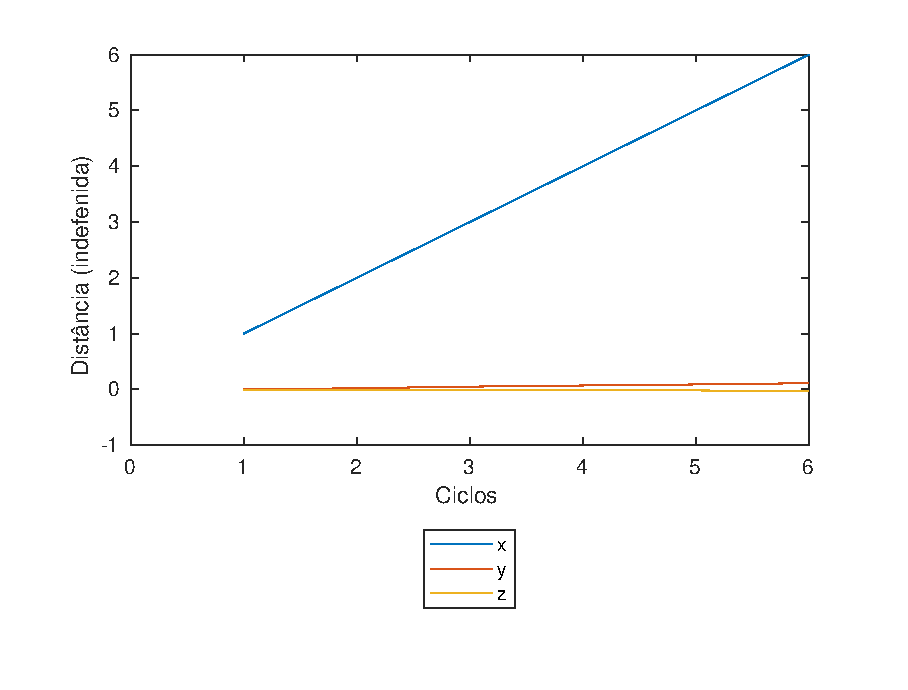
\includegraphics[width=0.45\textwidth]{testes/10cm_median/PositionViso.eps}}
	\caption{Coordenadas x, y e z do robô no movimento de 10 cm frente. a) Odometria Visual movimento lento b) Odometria Visual movimento rápido.}
	\label{fig:pos10cm}
\end{figure}


Numa análise de posição (x e y), a figura ~\ref{fig:traj10cm} ilustra o deslocamento efetuado e as diferenças entre as velocidades do movimento. Numa representação 3D (x,y,z), figura ~\ref{fig:traj3D10cm}, é notória a falta de um fator escala entre ciclos para obter um valor real, em metros, do movimento.  O mesmo pode ser justificado pelo facto de num  movimento mais rápido a diferença entre imagens capturadas é superior ao movimento mais lento. 


\begin{figure}[h!]
	\centering
	\subfloat[\label{fig:trajViso10cmslow}]{
		\includegraphics[width=0.45\textwidth]{testes/10cm_slow/Trajetoria.eps}}
	\qquad
	\subfloat[\label{fig:trajOdo10cmmedian}]{
		\includegraphics[width=0.45\textwidth]{testes/10cm_median/Trajetoria.eps}}
	\caption{Trajetória do robô no movimento de 10 cm frente. a) Odometria Visual movimento lento b) Odometria Visual movimento rápido.}
	\label{fig:traj10cm}
\end{figure}




\begin{figure}[h!]
	\centering
	\subfloat[\label{fig:traj3DViso10cmslow}]{
		\includegraphics[width=0.45\textwidth]{testes/10cm_slow/Trajetoria3D.eps}}
	\qquad
	\subfloat[\label{fig:traj3DViso10cmmedian}]{
		\includegraphics[width=0.45\textwidth]{testes/10cm_median/Trajetoria3D.eps}}
	\caption{Trajetória 3D do robô no movimento de 10 cm frente. a) Odometria Visual movimento lento b) Odometria Visual movimento rápido.}
	\label{fig:traj3D10cm}
\end{figure}




\FloatBarrier
Desta forma, nos próximos testes a escala obtida na Odometria Visual não têm unidade devido ao movimento ter velocidades sempre diferentes, tanto no mesmo movimento como em movimentos diferentes. 



\FloatBarrier
\subsubsection{Frente e Tràs}\label{subsubsection:EmFrenteTraz}

Neste teste o robô desloca-se cerca de 3 metros em frente e 2 metros para tràs, movimento na coordenada de x. A trajetória resultante é representada na figura ~\ref{fig:trajRobo3mFrente2mTraz}, em que na  Odometria das rodas do robô a coordenada x evolui até aos 3 metros e de seguida diminui até ao 1 metro. Por outro lado,  na Odometria Visual esta evolui até um ponto 20 (escala indefinida) e de seguida diminui até o ponto 5 (escala indefinida), como ilustrado na figura ~\ref{fig:pos3mFrente2mTraz}.


\begin{figure}[h!]
	\begin{center}
		\leavevmode		
		\includegraphics[width=0.65\textwidth]{testes/3mFrente2mTraz/Trajetoria.eps}
		\caption{Trajetória do robô no movimento frente e tràs.}
		\label{fig:trajRobo3mFrente2mTraz}
	\end{center}
\end{figure}



\begin{figure}[h!]
	\centering
	\subfloat[\label{fig:posViso3mFrente2mTraz}]{
		\includegraphics[width=0.45\textwidth]{testes/3mFrente2mTraz/PosicaoViso.eps}}
	\qquad
	\subfloat[\label{fig:posOdoEst2mTraz}]{
		\includegraphics[width=0.45\textwidth]{testes/3mFrente2mTraz/PosicaoOdo.eps}}
	\caption{Coordenadas x, y e z do robô  no movimento frente e tràs. a) Odometria Visual e b) Odometria das rodas do robô.}
	\label{fig:pos3mFrente2mTraz}
\end{figure}

De realçar que o valor máximo da coordena x obtida foi 20 e a distância percorrida foram 3 metros tal e qual o teste anterior,subcapítulo ~\ref{subsubsection:EmFrente} . Esta diferença deve-se a diferença de velocidades nos testes.


Em relação aos ângulos, estes mantêm-se constantes e nulos, como ilustrado na figura ~\ref{fig:ang3mFrente2mTraz}. As variações do ângulo $\gamma$ já foram justificadas anteriormente.


\begin{figure}[h!]
	\centering
	\subfloat[\label{fig:angViso3mFrente2mTraz}]{
		\includegraphics[width=0.45\textwidth]{testes/3mFrente2mTraz/AnglesViso.eps}}
	\qquad
	\subfloat[\label{fig:angOdo3mFrente2mTraz}]{
		\includegraphics[width=0.45\textwidth]{testes/3mFrente2mTraz/AnglesOdo.eps}}
	\caption{Angulos $\alpha$, $\beta$ e $\gamma$ do robô  no movimento frente e tràs. a) Odometria Visual e b) Odometria das rodas do robô.}
	\label{fig:ang3mFrente2mTraz}
\end{figure}


\FloatBarrier
\subsection{Movimento angular}\label{subsubsection:Rotacao}

Neste teste o robô é sujeito a uma velocidade angular para rodar sobre si próprio num ângulo apenas. Desta forma, pretende-se que o robô mantenha a sua posição e aumente o valor de um ângulo. O teste realizado foi a rotação de 90 graus .


\FloatBarrier
\subsubsection{90 graus}\label{subsubsection:Rotacao90}


Neste teste o robô realiza uma rotação sobre si próprio de 90 graus. Na figura ~\ref{fig:trajRoboRot90} está representada a trajetória resultante do movimento. 

\begin{figure}[h!]
	\begin{center}
		\leavevmode		
		\includegraphics[width=0.65\textwidth]{testes/rotacao90/Trajetoria.eps}
		\caption{Trajetória do robô no movimento angular de 90 gruas.}
		\label{fig:trajRoboRot90}
	\end{center}
\end{figure}


Em análise mais detalhada, figura ~\ref{fig:posRot90}, a Odometria das rodas do robô  apresenta uma variação pequena da posição, praticamente nula, e a Odometria Visual mostra maior erro, causando grandes variações na posição. 

\begin{figure}[h!]
	\centering
	\subfloat[\label{fig:posVisoRot90}]{
		\includegraphics[width=0.45\textwidth]{testes/rotacao90/PosicaoViso.eps}}
	\qquad
	\subfloat[\label{fig:posOdoRot90}]{
		\includegraphics[width=0.45\textwidth]{testes/rotacao90/PosicaoOdo.eps}}
	\caption{Coordenadas x, y e z do robô  no movimento angular de 90 gruas. a) Odometria Visual e b) Odometria das rodas do robô.}
	\label{fig:posRot90}
\end{figure}


Estes erros são originados por pequenos movimentos da câmara e/ou robô,que influenciam a imagem e causam um erro na translação, como é ilustrado na figura ~\ref{fig:ExplicPosErr}. Esta, é composta pela imagem anterior \textit{frame} \textit{k-1} à esquerda e pela imagem atual \textit{frame} \textit{k} à direita. Cada imagem tem representa a coordenada do ponto característico que é correspondente nas imagens. De notar que as imagens estão concatenadas e por isso, os valores dos pixeis da segunda imagem estão afetados pela largura da primeira imagem. Visto ter sido realizado um movimento angular um píxel na imagem devia apenas se alterar na coordenada \textbf{X} e manter sempre o mesmo valor da coordenada \textbf{Y}, como ilustrado na figura ~\ref{fig:ExplicPosErrCerto}.



\begin{figure}[h!]
	\begin{center}
		\leavevmode		
		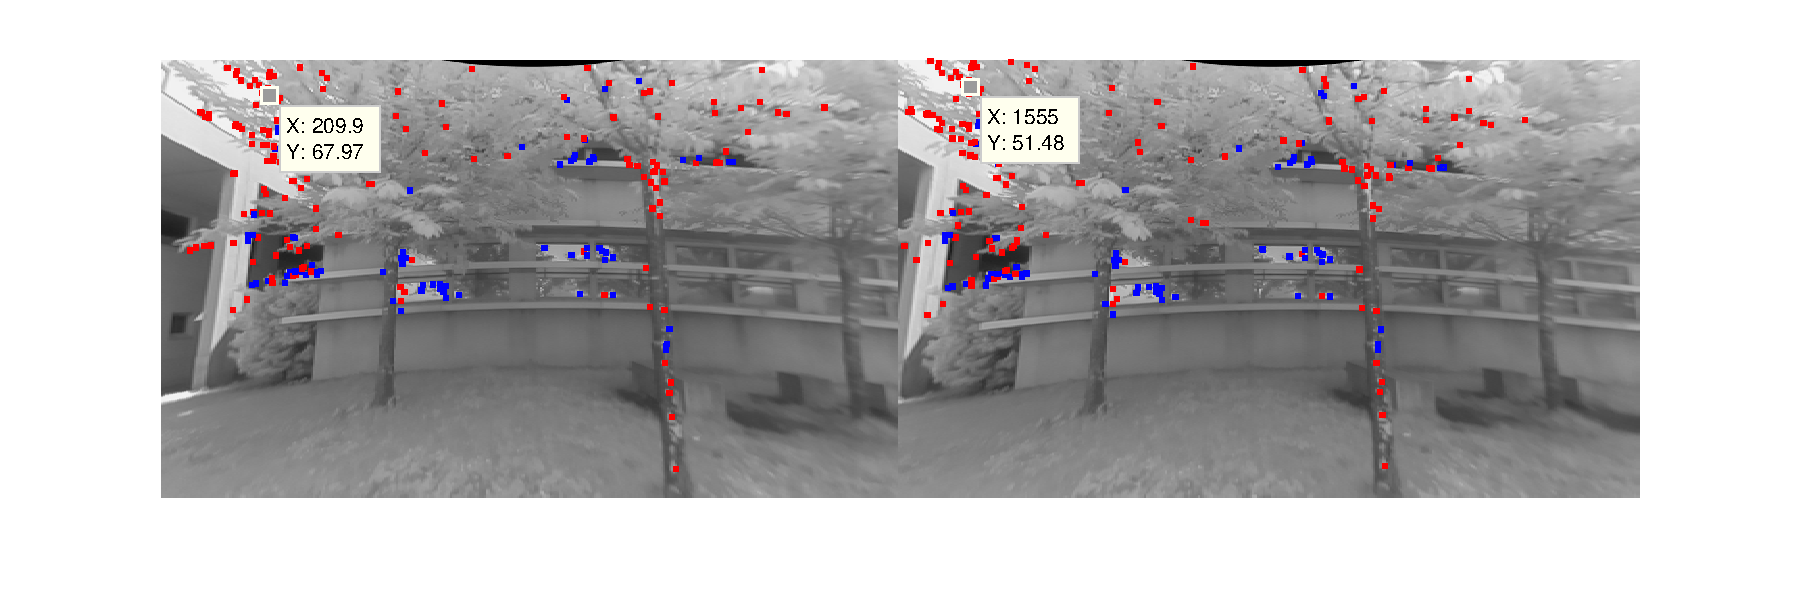
\includegraphics[width=1\textwidth]{testes/rotacao90/ExplicacaoPosErro.eps}
		\caption{Distribuição dos pontos característicos da imagem anterior \textit{k-1} e a atual \textit{k}.}
		\label{fig:ExplicPosErr}
	\end{center}
\end{figure}


\begin{figure}[h!]
	\begin{center}
		\leavevmode		
		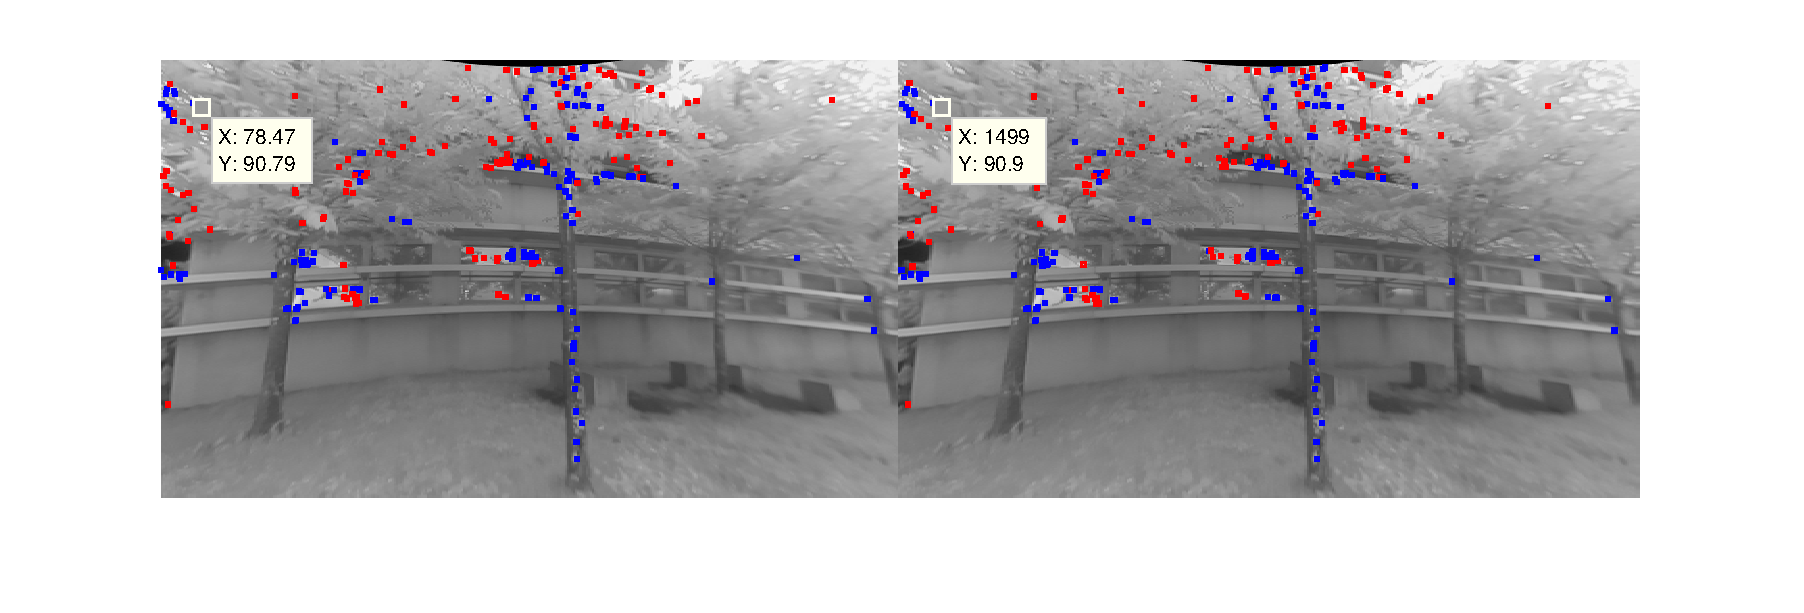
\includegraphics[width=1\textwidth]{testes/rotacao90/ExplicacaoPosErroCerto.eps}
		\caption{Distribuição dos pontos característicos da imagem anterior \textit{k-1} e a atual \textit{k}.}
		\label{fig:ExplicPosErrCerto}
	\end{center}
\end{figure}


Em relação aos ângulos, representados na figura ~\ref{fig:angRot90}, não são afetados pelos pormenores identificados em cima. De salientar, que o movimento realizado foi uma rotação de aproximadamente 15 graus, paragem na rotação (devido a problemas de comunicação entre o robô e o comando) e rotação até cerca de 90 graus. 


\begin{figure}[h!]
	\centering
	\subfloat[\label{fig:angVisoRot90}]{
		\includegraphics[width=0.45\textwidth]{testes/rotacao90/AnglesViso.eps}}
	\qquad
	\subfloat[\label{fig:angOdoRot90}]{
		\includegraphics[width=0.45\textwidth]{testes/rotacao90/AnglesOdo.eps}}
	\caption{Ângulos $\alpha$, $\beta$ e $\gamma$ do robô  no movimento angular de 90 gruas. a) Odometria Visual e b) Odometria das rodas do robô.}
	\label{fig:angRot90}
\end{figure}


O ângulo na Odometria das rodas do robô é representado na figura ~\ref{fig:angOdoRot90} e tem o comportamento desejado. Em relação à figura ~\ref{fig:angVisoRot90}, Odometria Visual, evolui inicialmente como desejado mas perto do ciclo 25 é detetada uma variação errada, que causa erros na solução final. Este erro é causado pela errada correspondência de pontos característicos, como ilustrada a figura ~\ref{fig:ExplicAngErr}. 


\begin{figure}[h!]
	\begin{center}
		\leavevmode		
		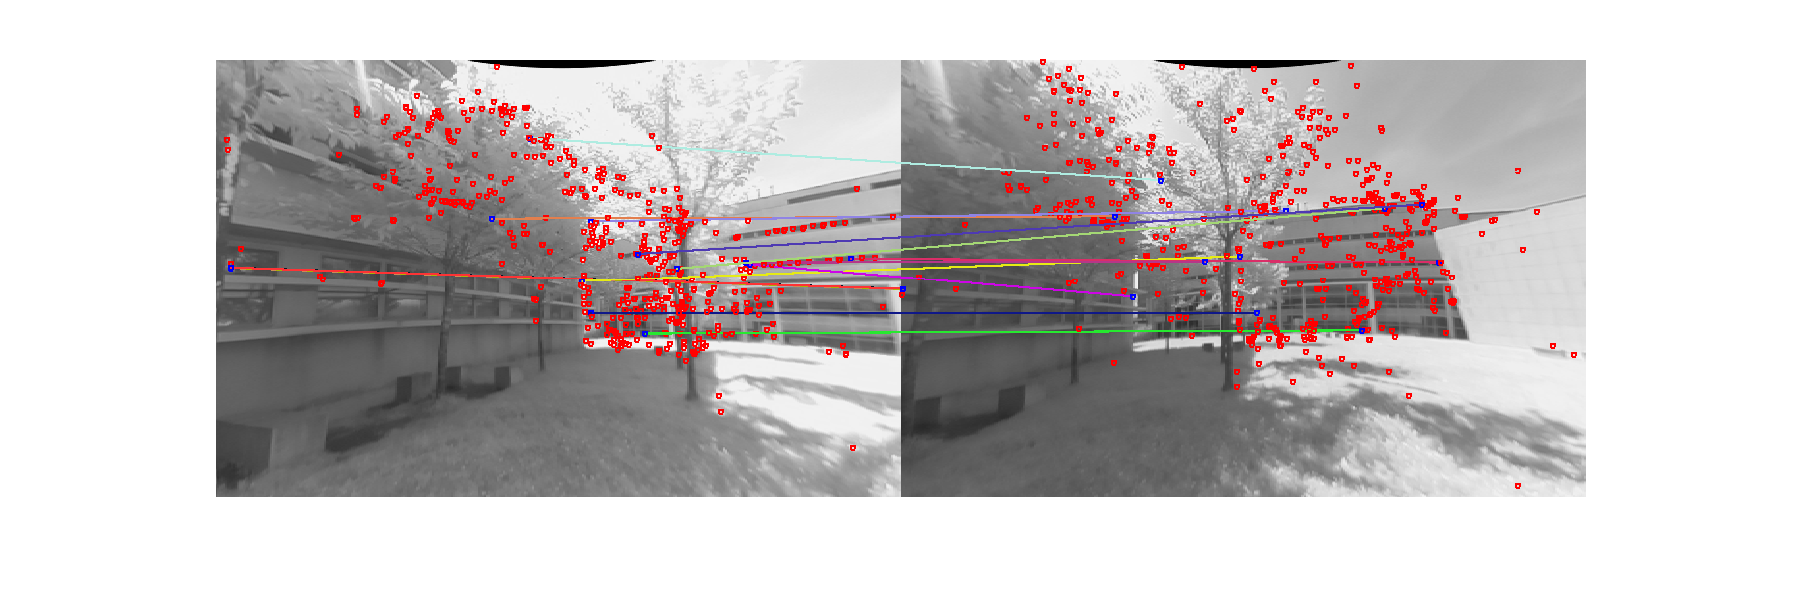
\includegraphics[width=1\textwidth]{testes/rotacao90/ExplicacaoAngErro.eps}
		\caption{Errada correspondência dos pontos caracteristicos da imagem anterior \textit{k-1} e a atual \textit{k}.}
		\label{fig:ExplicAngErr}
	\end{center}
\end{figure}


A figura ~\ref{fig:AnglesErro} representa a diferença entre os ângulos $\alpha$, $\theta$ e $\gamma$ da Odometria das rodas do robô e da Odometria Visual. Inicialmente, existe um pequeno erro em $\beta$ e $\alpha$. Em $\beta$ devido a mal correspondência, mas erro próximo de zero, enquanto em $\alpha$ desce ao tempo de processamento que inicialmente causa essa diferença, mas depois ajusta. Na zona do ciclo 25, mais precisamente no ciclo 27, a variação do erro é brusca em todos os ângulos, isto devido à situação explícita anteriormente. De salientar, que o erro causado no ângulo $\alpha$ não foi significativo e desta forma o erro consegue convergir para zero.



\begin{figure}[h!]
	\begin{center}
		\leavevmode		
		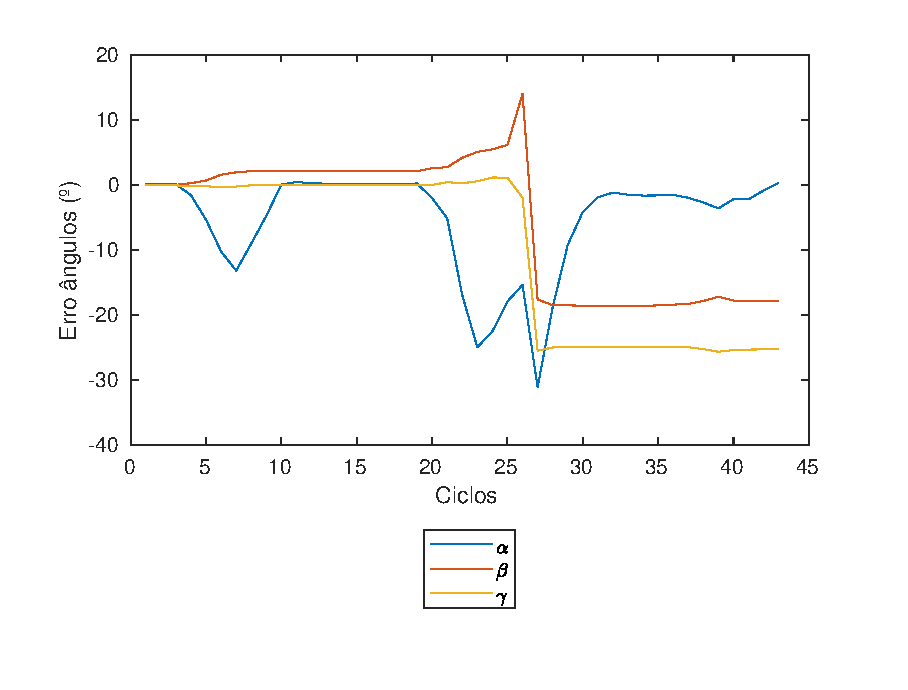
\includegraphics[width=.8\textwidth]{testes/rotacao90/AnglesErro.eps}
		\caption{Erro entre os ângulos da Odometria das rodas do robô e a Odometria Visual no movimento angular de 90 gruas.}
		\label{fig:AnglesErro}
	\end{center}
\end{figure}



\FloatBarrier
\subsection{Movimento em L (semi-quadrado)}\label{subsubsection:L}


O movimento em semi-quadrado é composto pelo movimento em frente, neste teste 3 metros, rotação de 90 graus sobre si próprio e outro movimento em frente, 1 metro.

A figura ~\ref{fig:trajRobo3m1mL_2} ilustra o movimento deste teste. A  azul é representado o movimento do robô com base na Odometria das rodas e a amarelo é a Odometria Visual, sendo esta última constituída por um erro na rotação, devido a fatores explícitos no subcapítulo ~\ref{subsubsection:Rotacao90}. Devido à Odometria das rodas ter uma orientação dos eixos diferente da Odometria Visual faz com que a rotação seja no sentido inverso e dessa forma o movimento em semi-quadrado tenha representações diferentes.

\pagebreak

\begin{figure}[h!]
	\begin{center}
		\leavevmode		
		\includegraphics[width=0.65\textwidth]{testes/3m1mL_2/Trajetoria.eps}
		\caption{Trajetória do robô no movimento semi-quadrangular.}
		\label{fig:trajRobo3m1mL_2}
	\end{center}
\end{figure}



Analisando ao pormenor o deslocamento nas diferentes direções, como ilustrado na figura ~\ref{fig:pos3m1mL_2}, conclui-se que os movimentos em x e y são semelhantes, sendo y o inverso na Odometria Visual da Odometria das rodas devido às diferenças entre os eixos base. Em relação ao movimento em z, este apresenta um pequeno erro no final causado pelos ângulos de rotação.

\begin{figure}[h!]
	\centering
	\subfloat[\label{fig:posViso3m1mL_2}]{
		\includegraphics[width=0.45\textwidth]{testes/3m1mL_2/PosicaoViso.eps}}
	\qquad
	\subfloat[\label{fig:posOdo3m1mL_2}]{
		\includegraphics[width=0.45\textwidth]{testes/3m1mL_2/PosicaoOdo.eps}}
	\caption{Coordenadas x, y e z do robô  no movimento semi-quadrangular. a) Odometria Visual e b) Odometria das rodas do robô.}
	\label{fig:pos3m1mL_2}
\end{figure}


Como ilustrado na figura ~\ref{fig:ang3m1mL_2}, o erro na variação dos ângulos, perto do ciclo 80, afeta a trajetória final. Este erro é derivado de uma má correspondência de pontos característicos, pelo facto de ter rotação da câmara ter sido muito brusca, causando uma grande distância angular entre imagens consecutivas.


\begin{figure}[h!]
	\centering
	\subfloat[\label{fig:angViso3m1mL_2}]{
		\includegraphics[width=0.45\textwidth]{testes/3m1mL_2/AnglesViso.eps}}
	\qquad
	\subfloat[\label{fig:angOdo3m1mL_2}]{
		\includegraphics[width=0.45\textwidth]{testes/3m1mL_2/AnglesOdo.eps}}
	\caption{Angulos $\alpha$, $\beta$ e $\gamma$ do robô  no movimento semi-quadrangular. a) Odometria Visual e b) Odometria das rodas do robô.}
	\label{fig:ang3m1mL_2}
\end{figure}

\pagebreak

A figura ~\ref{fig:ExplicAngErr3m1mL_2} representa a imagem anterior e a corrente no instante de ciclo 73, precisamente onde acontece o erro nos ângulos. Nesta imagem é possível observar uma diferença grande de rotação, originando poucas correspondências de pontos característicos e pelo menos uma correspondência errada, segmento de reta a preto.

\begin{figure}[h!]
	\begin{center}
		\leavevmode		
		\includegraphics[width=1\textwidth]{testes/3m1mL_2/ExplicacaoERROAngle.eps}
		\caption{Correspondência de pontos característicos com maior rotação do robô.}
		\label{fig:ExplicAngErr3m1mL_2}
	\end{center}
\end{figure}


A figura ~\ref{fig:Traj3D3m1mL_2} representa a trajetória 3D do robô. Esta tem representado os eixos de orientação e o número correspondente a cada ciclo. O inicio é na posição (0,0,0) e o movimento inicial é sobre o eixo x, eixo vermelho. Ao chegar perto do ponto de rotação os eixos efetuam a devida rotação e de seguida prossegue o movimento em frente terminando a trajetória no ponto (21,-12,14). 

Nesta figura é possível a análise do erro causado pelo ângulo z. Devido a este ter obtido um valor diferente de nulo causa um movimento também no eixo do z.

\begin{figure}[h!]
	\begin{center}
		\leavevmode		
		\includegraphics[width=.8\textwidth]{testes/3m1mL_2/Trajetoria3D.eps}
		\caption{Trajetória 3D do robô no movimento semi-quadrangular.}
		\label{fig:Traj3D3m1mL_2}
	\end{center}
\end{figure}






\FloatBarrier
\subsection{Movimento quadrangular}\label{subsubsection:Quadrado}


Por último resta elaborar o teste do movimento quadrangular. Neste teste, pretende-se que o robô realize um quadrado de 1 metro de largura e no final a sua posição seja igual à posição inicial.

Como ilustrado na figura ~\ref{fig:trajRobo1mquadrado}, a azul está representado a trajetória do robô obtida pela Odometria das rodas do robô, enquanto a amarelo é representada a Odometria Visual. 


\begin{figure}[h!]
	\begin{center}
		\leavevmode		
		\includegraphics[width=0.65\textwidth]{testes/1mquadrado/Trajetoria.eps}
		\caption{Trajetória do robô no movimento em quadrangular.}
		\label{fig:trajRobo1mquadrado}
	\end{center}
\end{figure}


A Odometria Visual não realiza um quadrado perfeito mas, removendo as zonas de rotação é de salientar os quatro movimentos realizados:
\begin{itemize}
 	\item movimento em frente, aumento da coordenada x inicialmente.
 	\item movimento em frente com rotação de 90 graus, aumento da coordenada y.
 	\item movimento em frente com rotação de 180 graus, diminui a coordenada x.
 	\item movimento em frente com rotação de 270 graus, diminui a coordenada y.
\end{itemize}

Estes movimentos são ilustrados na figura ~\ref{fig:posViso1mquadrado} mas com alguns erros nas zonas de rotação. Comparando as figuras ilustradas na figura ~\ref{fig:pos1mquadrado}, as diferenças são que o movimento y toma valores negativos na Odometria das rodas do robô e na Odometria Visual valores positivos. Tal, deve-se à definição dos referências iniciais, estando o eixo y oposto. Outra diferença é a quantidade de erro existente na Odometria Visual nas rotações.


\begin{figure}[h!]
	\centering
	\subfloat[\label{fig:posViso1mquadrado}]{
		\includegraphics[width=0.45\textwidth]{testes/1mquadrado/PosicaoViso.eps}}
	\qquad
	\subfloat[\label{fig:posOdo1mquadrado}]{
		\includegraphics[width=0.45\textwidth]{testes/1mquadrado/PosicaoOdo.eps}}
	\caption{Coordenadas x, y e z do robô  no movimento em Frente e Tràs. a) Odometria Visual e b) Odometria das rodas do robô.}
	\label{fig:pos1mquadrado}
\end{figure}


Em termos de ângulos, a figura ~\ref{fig:ang1mquadrado} representa a evolução dos ângulos das diferentes Odometrias. O erro entre os ângulos é representado na figura ~\ref{fig:anglesERROquad}. De analisar que o erro varia pouco, havendo apenas picos de variação quando os ângulos atingem valores de 180 graus e -180 graus. No final da trajetória é encontrado um obstáculo móvel, que resulta no erro da variação do ângulo errado. 


\begin{figure}[h!]
	\centering
	\subfloat[\label{fig:angViso1mquadrado}]{
		\includegraphics[width=0.45\textwidth]{testes/1mquadrado/AnglesViso.eps}}
	\qquad
	\subfloat[\label{fig:angOdoRot180}]{
		\includegraphics[width=0.45\textwidth]{testes/1mquadrado/AnglesOdo.eps}}
	\caption{Angulos $\alpha$, $\beta$ e $\gamma$ do robô  no movimento quadrangular. a) Odometria Visual e b) Odometria das rodas do robô.}
	\label{fig:ang1mquadrado}
\end{figure}

\begin{figure}[h!]
	\begin{center}
		\leavevmode		
		\includegraphics[width=0.8\textwidth]{testes/1mquadrado/AnglesERRo.eps}
		\caption{Erro dos ângulos $\alpha$, $\beta$ e $\gamma$ entre a Odometria Visual e a Odometria das rodas do robô.}
		\label{fig:anglesERROquad}
	\end{center}
\end{figure}



%\begin{figure}[h!]
%	\begin{center}
%		\leavevmode		
%		\includegraphics[width=0.8\textwidth]{testes/1mquadrado/Trajetoria3D_2.eps}
%		\caption{Trajetória 3D do robô no movimento quadrangular.}
%		\label{fig:traj3DRobo1mquadrado}
%	\end{center}
%\end{figure}


\section{Análise Geral de Resultados}


Nesta secção será apresentado um resumo dos resultados obtidos. 

A calibração da câmara é essencial para remoção da distorção da imagem. Esta distorção afeta a imagem e causa erros nas correspondências devido à falta de nitidez nas bermas da imagem, zona de maior distorção. Desta forma, e com um script desenvolvido em Matlab é obtida a matriz intrínseca e de parâmetros de distorção, utilizadas para remover a zona de maior distorção da imagem e efeitos de olho de peixe. A imagem final obtida para análise é uma imagem com ângulo de abertura entre a imagem sem lente e a imagem com lente olho de peixe \textit{full-frame}. 

Em termos dos detetores de características, nesta dissertação foram utilizados 4 dos quais 2, SIFT e HARRIS não são ideais para o meio envolvido e os outros 2, FAST e SURF são mais indicados devido à sua boa distribuição dos pontos característicos pela zonas de vinha, quantidade e correspondência.

Em relação às combinações dos detetores, descritores e matchers foram comparados vários parâmetros tais como tempo de ciclo, imagens processadas, imagens perdidas entre ciclos e número de características de 24 combinações possíveis. Assim, as combinações SURF/ORB/FLANN e FAST/ORB/FLANN são as que obtêm melhores resultados sendo a primeira combinação a utilizadas nos testes realizados.

Relativamente aos testes realizados, estes comparam a Odometria Visual com a Odometria de rodas do robô, obtida através de um tópico já desenvolvido no ROS do Agrobv16 com base na cinemática diferencial. Os percursos realizados foram efetuados, em que o percurso seguinte é baseado no percurso anterior com a adição de uma nova característica a testar. Desta forma, os percursos realizados foram : estático, movimento em linha reta, movimento angular, movimento em semi-quadrangular e movimento quadrangular.


O teste estático é realizado para comprovar que a posição e os ângulos do robô se mantêm sempre estáticos. O movimento em linha reta prevê mostrar que num movimento em frente, apenas se modifica uma coordenada da posição do robô, mantendo-se os ângulos. De forma a validar o movimento oposto é realizado um teste de frente e tràs, demonstrando que a coordenada do robô aumenta e diminui. E, ainda,  que quando existe essa variação os ângulos se mantêm constantes. No que diz respeito, ao movimento angular, este tem como objetivo mostra que numa rotação do robô sobre si próprio apenas varia o valor de um ângulo e robô mantêm a sua posição estável, sem movimentos. Numa junção de testes anteriores é realizado o percurso semi-quadrangular de forma, a variar 2 coordenadas de posição e o valor de um ângulo. Por fim, é testado o movimento quadrangular com objetivo de o robô partir de um ponto inicial e terminar a trajetória nesse mesmo ponto, realizando 4 movimentos lineares e 4 rotações.

 
Ao longo da realização dos testes foram detetados alguns erros que podem ser justificados por várias situações.No teste do movimento linear não foi possível realizar uma comparação direta entre Odometria Visual e de rodas do robô, uma vez que não foi possível produzir resultados em metros tal como é ilustrativo em Odometria Visual.


Quanto ao movimento angular verificou-se alguns erros uma vez que o robô realizada um movimento brusco que afeta a cabeça  do robô (topo de robô). Além disso, o movimento brusco provoca rotações muito rápidas rotações grandes entre imagens consecutivas provocando combinações erradas de pontos característicos entre imagens.


Na conjugação destes movimentos são obtidos erros dependentes dos anteriores, tais como, no movimento em semi-quadrangular a rotação tem deslocamento que deveria de ser nulo, o que não foi possível verificar. O mesmo acontece no movimento quadrangular.


Em suma, é possível analisar o movimento pretendido graficamente e rotações corretas quando o movimento é constante. Quando este se torna rápido os resultados alteram-se originando erros. 

